\documentclass[12pt,a4paper,oneside]{report} %<<<1 ------------------------------
% fonty, kodovani:
\usepackage[utf8]{inputenc}             % soubor je v utf8:
\usepackage{cmap}                       % preklad kodovani aby pdfko bylo kopirovatelne se spravnymi cs znaky, musi byt vhodny font, viz dalsi 2 radky
\usepackage[T1]{fontenc}                % viz ^
\usepackage{tgtermes}                   % kvalitni font times, ktery je v pdf kopirovatelny i s cs znaky viz ^^
\usepackage{textcomp}                   % spravne stojate mikro pro SI prefix, pouziti: \textmu, ve vzorci: $\hbox{\textmu}$
\usepackage{slantsc}                   % spravne stojate mikro pro SI prefix, pouziti: \textmu, ve vzorci: $\hbox{\textmu}$
\usepackage{calc}                   % provides \widthof
\usepackage{enumitem}                   % provides \begin{description} with settings []
\usepackage{color}                   % provides colour text
% obrazky:
\usepackage{graphicx}                   % vlozeni obrazku
\usepackage{grffile}                    % umoznuje mezery v nazvech souboru obrazku
\grffilesetup{ multidot=false, babel=false, encoding, inputencoding=utf8, filenameencoding=utf8, space=true}
\newcommand*{\FILEDOT}{.}                   % pokud obrazek v souboru s teckou (napr. aaa.bbb.pdf), pak si TeX mysli ze to uz je pripona, musi % se tecka obejit timhle: \includegraphics{aaa\FILEDOT bbb.eps}
% ostatni:
\usepackage[pdftex,
            unicode,
            pdfauthor={Q-Wave consorcium},
            pdftitle={Quantum Wave ToolBox documentation},
            pdfkeywords={algorithm, data procesing, sampling, toolbox},
            pdfproducer={Latex with hyperref},
            pdfcreator={pdflatex}]{hyperref}
%\usepackage[a4paper]{geometry}          % zajisti A4
%\geometry{verbose,lmargin=2.5cm,rmargin=2.5cm,tmargin=2.5cm,bmargin=2.5cm}      % nastaveni okraju
\usepackage{url}                        % moznost parametru url v bibtexu
%\usepackage{setspace} \doublespacing   % dvojite radkovani, pokud 1.5 pak \onehalfspace
\usepackage{xspace}
\usepackage{amsmath}                    % 
\usepackage{color}

% lstlisting settings %<<<1 ----------------------------------------------------
\usepackage{listings}
\definecolor{mygreen}{rgb}{0,0.6,0}
\definecolor{mygray}{rgb}{0.5,0.5,0.5}
\definecolor{lightgray}{rgb}{0.95,0.95,0.95}
\definecolor{mymauve}{rgb}{0.58,0,0.82}

\lstdefinestyle{mcode}{
%\lstset{ %
  backgroundcolor=\color{lightgray},   % choose the background color; you must add \usepackage{color} or \usepackage{xcolor}
  basicstyle=\normalsize\sffamily,        % the size of the fonts that are used for the code
  breakatwhitespace=false,         % sets if automatic breaks should only happen at whitespace
  breaklines=true,                 % sets automatic line breaking
  captionpos=b,                    % sets the caption-position to bottom
  commentstyle=\color{mygreen},    % comment style
  deletekeywords={...},            % if you want to delete keywords from the given language
  escapeinside={\%*}{*)},          % if you want to add LaTeX within your code
  extendedchars=true,              % lets you use non-ASCII characters; for 8-bits encodings only, does not work with UTF-8
  frame=single,	                   % adds a frame around the code
  keepspaces=true,                 % keeps spaces in text, useful for keeping indentation of code (possibly needs columns=flexible)
  keywordstyle=\color{blue},       % keyword style
  language=Matlab,                 % the language of the code
  otherkeywords={*,qwtb,alg_info,alg_wrapper,
        normrnd, alg_test,alg_example,...},           % if you want to add more keywords to the set
  numbers=none,                    % where to put the line-numbers; possible values are (none, left, right)
  numbersep=5pt,                   % how far the line-numbers are from the code
  numberstyle=\tiny\color{mygray}, % the style that is used for the line-numbers
  rulecolor=\color{black},         % if not set, the frame-color may be changed on line-breaks within not-black text (e.g. comments (green here))
  showspaces=false,                % show spaces everywhere adding particular underscores; it overrides 'showstringspaces'
  showstringspaces=false,          % underline spaces within strings only
  showtabs=false,                  % show tabs within strings adding particular underscores
  stepnumber=2,                    % the step between two line-numbers. If it's 1, each line will be numbered
  stringstyle=\color{mymauve},     % string literal style
  tabsize=2,                       % sets default tabsize to 2 spaces
  title=\lstname,                  % show the filename of files included with \lstinputlisting; also try caption instead of title
  belowskip=0pt                  % skip after end of lstlistings
}

\lstdefinestyle{output}{
%\lstset{ %
  backgroundcolor=\color{lightgray},   % choose the background color; you must add \usepackage{color} or \usepackage{xcolor}
  basicstyle=\normalsize\itshape,        % the size of the fonts that are used for the code
  breakatwhitespace=false,         % sets if automatic breaks should only happen at whitespace
  breaklines=true,                 % sets automatic line breaking
  captionpos=b,                    % sets the caption-position to bottom
  commentstyle=\color{mygreen},    % comment style
  deletekeywords={...},            % if you want to delete keywords from the given language
  escapeinside={\%*}{*)},          % if you want to add LaTeX within your code
  extendedchars=true,              % lets you use non-ASCII characters; for 8-bits encodings only, does not work with UTF-8
  frame=none,	                   % adds a frame around the code
  keepspaces=true,                 % keeps spaces in text, useful for keeping indentation of code (possibly needs columns=flexible)
  keywordstyle=\color{blue},       % keyword style
  language=Matlab,                 % the language of the code
  otherkeywords={*,qwtb,alg_info,alg_wrapper,alg_test,alg_example,...},           % if you want to add more keywords to the set
  numbers=none,                    % where to put the line-numbers; possible values are (none, left, right)
  numbersep=5pt,                   % how far the line-numbers are from the code
  numberstyle=\tiny\color{mygray}, % the style that is used for the line-numbers
  rulecolor=\color{black},         % if not set, the frame-color may be changed on line-breaks within not-black text (e.g. comments (green here))
  showspaces=false,                % show spaces everywhere adding particular underscores; it overrides 'showstringspaces'
  showstringspaces=false,          % underline spaces within strings only
  showtabs=false,                  % show tabs within strings adding particular underscores
  stepnumber=2,                    % the step between two line-numbers. If it's 1, each line will be numbered
  stringstyle=\color{mymauve},     % string literal style
  tabsize=2,                       % sets default tabsize to 2 spaces
  title=\lstname,                  % show the filename of files included with \lstinputlisting; also try caption instead of title
  belowskip=0pt,                  % skip after end of lstlistings
  xleftmargin=20pt                      % margin on left side
}

\lstset{style=mcode}


% bibliography settings %<<<1 ----------------------------------------------------
\usepackage[english]{babel} % main language of the document must be last
\usepackage[
   backend=biber      % if we want unicode 
  ,style=ieee   % or iso-numeric for numeric citation method          
  ,babel=other        % to support multiple languages in bibliography
  %,sortlocale=cs_CZ   % locale of main language, it is for sorting
  ,sortlocale=en_UK   % locale of main language, it is for sorting
  ,bibencoding=UTF8   % this is necessary only if bibliography file is in different encoding than main document
]{biblatex}

\bibliography{alllib2}
%\defbibenvironment{bibliography}
%    {\list
%        {[\printfield[labelnumberwidth]{labelnumber}]}
%        {\setlength{\labelwidth}{\labelnumberwidth}
%        \setlength{\leftmargin}{4pt}
%        \setlength{\labelsep}{10pt}
%        \addtolength{\leftmargin}{\labelsep}
%        \setlength{\itemsep}{6pt}
%        \setlength{\parsep}{\bibparsep}}
%        \renewcommand*{\makelabel}[1]{\hss##1}}
%    {\endlist}
%    {\item}

% zkratky %<<<1 ----------------------------------------------------

\def\Alg{{\sc Algorithm}\xspace}
\def\Algs{{\sc Algorithms}\xspace}
\def\Tb{{\sc Toolbox}\xspace}
\def\Da{{\sc Data}\xspace}
\def\Mea{{\sc Measurement}\xspace}
\def\Qua{{\sc Quantity}\xspace}
\def\Quas{{\sc Quantities}\xspace}
\def\Wr{{\sc Wrapper}\xspace}
\def\Wrs{{\sc Wrappers}\xspace}
\def\matlab{{\sc MATLAB}\xspace}
\def\octave{{\sc GNU Octave}\xspace}
\def\labview{{\sc LabVIEW}\xspace}
\def\mgo{\matlab/\octave\xspace}
        
\begin{document} % dalsi nastaveni dokumentu --------------------------------------------%<<<1
% jak rozdelit specialni slova, napr.: au-to-ma-ti-za-ce
\hyphenation{Frame-work OpenOffice SourceForge Windows vstu-pních pra-vdě-po-do-bno-stní roz-dě-le-ní me-ze pra-vdě-po-do-bnost pra-vdě-po-do-bnos-tí
pse-u-do-ná-hod-ná pse-u-do-ná-hod-ných kan-ce-lář-ských ro-vno-měr-né}
%\def\thesection{\Roman{section}}       % redefinovani stylu cislovani sekce
\renewcommand\floatpagefraction{.9} \renewcommand\topfraction{.9} \renewcommand\bottomfraction{.9} \renewcommand\textfraction{.1} \setcounter{totalnumber}{50} \setcounter{topnumber}{50} \setcounter{bottomnumber}{50} % pokud moc obrazku, tak zmeni nastaveni podilu textu/floatu:
\renewcommand{\labelitemi}{--}          % oddelovac itemu
\setlength{\unitlength}{1mm}            % standartni delka v prostredi picture


\newenvironment{tightdesc}{\begin{description}[itemsep=0pt]} 
                              {\end{description}}

\title{Quantum Wave ToolBox documentation}
\author{Q-Wave consorcium}

% prvni strana ----------------------------------------------------------------------- %<<<1 ------------------------------
\thispagestyle{empty}
\begin{center}

\includegraphics[width=0.3\textwidth]{sources/qwlogo.jpg}
\hfill

\includegraphics[width=0.3\textwidth]{sources/eurametlogo.jpg}

        \vspace{8em}
        {\huge
        Quantum Wave ToolBox\\
        documentation}\\

        \vfill
        {\Huge \color{red}{BETA version}}

        \vfill
        {\Large Q-Wave consortium}\\
        \today
        
        \bigskip
        contact: \texttt{msira@cmi.cz}

        \vfill
\end{center}
\newpage

\tableofcontents

\begin{abstract} %<<<1 ------------------------------
\bigskip
\begin{center}
        \parbox{0.7\textwidth}{\textit{Press a button with bold title AMPLITUDE\\
        \dots drink a coffee \dots\\
        and get the result}}
\end{center}

\bigskip
\noindent Quantum Wave Tool Box (QWTB) is a toolbox for evaluation of measured data. QWTB consist of data
processing algorithms from very different sources and unificating application interface. The toolbox
gives the possibility to use different data processing algorithms with one set of data and removes
the need to reformat data for every particular algorithm. Toolbox is extensible. The toolbox
can variate input data and calculate uncertainties by means of Monte Carlo Method
(MCM)~\cite{JCGM2008}.
\end{abstract}

\chapter{Basic description of the toolbox} %<<<1 ------------------------
\section{Toolbox overall scheme} %<<<2 ------------------------------
The basic scheme of the toolbox is following:
\begin{center}
        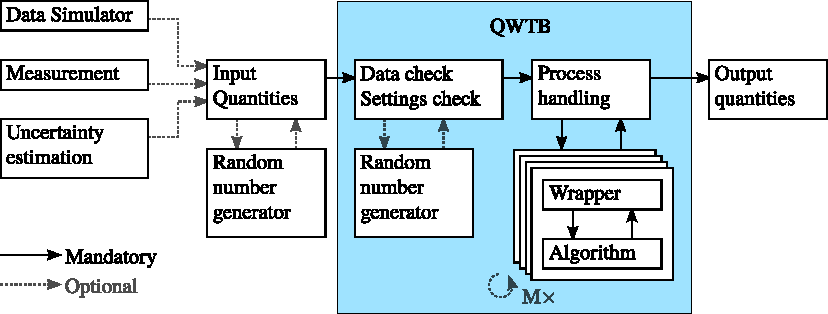
\includegraphics{sources/basic scheme v2.pdf}
\end{center}

User have to prepare the data, either based on a real measurement or simulated, into a specified
format. If needed, user can generate randomized data for selected quantities (e.g. with special
probability density functions) and prepare for Monte Carlo uncertainty calculation. Next user calls
toolbox to apply a selected algorithm on the data and review results. Toolbox will:
\begin{enumerate}
        \item Check user data.
        \item Check or generate calculation settings.
        \item If required, quantities are randomized according uncertainties to prepare for MCM uncertainty calculation.
        \item Data are handled to a wrapper. If needed, wrapper is run multiple times according MCM.
        \item Output data are the result of the toolbox.
\end{enumerate}

Another algorithm can be used immediately on the same data. User interface of the toolbox is represented
by the function \lstinline{qwtb} defined in the file {\tt qwtb.m}.

\section{Toolbox use} %<<<2 ------------------------------
The toolbox is used in several modes according to a number and character of input arguments.

\subsection{Get list of implemented algorithms} %<<<3
\begin{lstlisting}
alginfo = qwtb()
\end{lstlisting}

With no input arguments, toolbox returns informations on all available algorithms. Result array
\lstinline{alginfo} contains structures for every algorithm found in the same directory as
\texttt{qwtb.m}. Format of structures is defined in~\ref{structalginfo}.

\subsection{Application of an algorithm on the data} %<<<3 ------------------------------
\begin{lstlisting}
dataout = qwtb('algid', datain)
\end{lstlisting}

The algorithm is selected by first input argument \lstinline{algid}. It is a string with
designator of the algorithm, according structrue~\ref{structalginfo}.

The second input argument is the user data. Data have to be formatted in a structure with fields
named as quantities required by the algorithm (see~\ref{structquantity}).

The output variable is the structure with fields named as quantities.

In this case, standard calculation settings are used. If the user specifies calculation settings
in structure according~\ref{structcalcset}, it can be used as third input argument
\lstinline{calcset}:

\begin{lstlisting}
dataout = qwtb('algid', datain, calcset)
\end{lstlisting}

For some calculation settings some fields of \lstinline{datain} or \lstinline{calcset} are generated
automatically. To review automatically generated fields, user can get these structure in second and
third output argument:

\begin{lstlisting}
[dataout, datain, calcset] = qwtb('algid', datain)
[dataout, datain, calcset] = qwtb('algid', datain, calcset)
\end{lstlisting}

\subsection{Running an example of algorithm use} %<<<3 ------------------------------
Algorithm can have implemented an example of the use. This can be run by following syntax:

\begin{lstlisting}
[] = qwtb('algid', 'example')
\end{lstlisting}

The algorithm is selected by first input argument \lstinline{algid}. It is a string with
designator of the algorithm, according structrue~\ref{structalginfo}. The second argument is a
string. Toolbox will run a script \lstinline{alg_example.m} located in a algorithm directory.

After finish user can review input and output data or resulted figures if any.

\subsection{Running a test of algorithm} %<<<3 ------------------------------
Algorithm can have implemented a self test. This can be run by following syntax:

\begin{lstlisting}
[] = qwtb('algid', 'test')
\end{lstlisting}

The algorithm is selected by first input argument \lstinline{algid}. It is a string with
designator of the algorithm, according structrue~\ref{structalginfo}. The second argument is a
string. Toolbox will run a script \lstinline{alg_test.m} located in a algorithm directory.

Test should prepare data, run algorithm and check results. If implementation of algorithm
behaves incorrectly, an error will occur.

\subsection{Adding or removing algorithm path} %<<<3 ------------------------------
Algorithms are stored in different directories, which are not in \mgo load path. To add directory
with selected path to \mgo load path, following syntax is used:

\begin{lstlisting}
[] = qwtb('algid', 'addpath')
\end{lstlisting}

To remove path, use:

\begin{lstlisting}
[] = qwtb('algid', 'rempath')
\end{lstlisting}

Adding or removing path should be required only in special cases, such as debugging etc.

\chapter{Detailed description of the toolbox} %<<<1 ------------------------------
\section{Algorithm directory structure implementation} %<<<2 ------------------------------
Every algorithm is placed in a directory of following name:
\begin{center}
        {\tt alg\_X}
\end{center}
These directories have to be located in the directory containing the toolbox main script {\tt qwtb.m}.

Every algorithm directory contains following files:
\begin{tightdesc}
        \item [{\tt X1}, {\tt X2}, \dots] ---  Mandatory. One or more files with the algorithm itself.
        \item [{\tt alg\_info.m}] ---  Mandatory. Description of the algorithm. See \ref{filealginfo}.
        \item [{\tt alg\_wrapper.m}] ---  Mandatory. Wrapper of the algorithm. See \ref{filealgwrapper}.
        \item [{\tt alg\_test.m}] ---  Recomended. Testing function. See \ref{filealgtest}.
        \item [{\tt alg\_example.m}] ---  Recomended. Example script. See \ref{filealgexample}.
\end{tightdesc}

\subsection{File {\tt alg\_info.m}} %<<<3 ------------------------------
\label{filealginfo}
File contains a function with definition:

\begin{lstlisting}
function alginfo = alg_info()
\end{lstlisting}

The output \lstinline{alginfo} is a structure with informations about the algorithm. Structure is
defined in~\ref{structalginfo}.

File is mandatory. If file is missing in algorithm directory, QWTB will not recognize this
algorithm as part of the toolbox.

\subsection{File {\tt alg\_wrapper.m}} %<<<3 ------------------------------
\label{filealgwrapper}
File contains a function with definition:

\begin{lstlisting}
function dataout = alg_wrapper(datain, calcset)
\end{lstlisting}

The input \lstinline{datain} is a structure with input data (see %XXX
), \lstinline{calcset} is a structure with definition of calculation settings
(see~\ref{structcalcset}).
) and \lstinline{dataout} is a structure containing output data (see %XXX
).

The wrapper does following:
\begin{enumerate}
        \item Formats input data structure \lstinline{datain} into variables wuitable for algorithm.
        \item Runs the algorithm.
        \item Format results of the algorithm into data structure \lstinline{dataout}.
\end{enumerate}

File is mandatory. If file is missing in algorithm directory, QWTB will not recognize this
algorithm as part of the toolbox.

\subsection{File {\tt alg\_test.m}} %<<<3 ------------------------------
\label{filealgtest}
File contains a function with following definition:

\begin{lstlisting}
function [] = alg_test(calcset)
\end{lstlisting}

Test should generate sample data, run algorithm and check results by a function \lstinline{assert}.
QWTB will provide a standard calculation settings structure \lstinline{calcset} (see~\ref{structcalcset}).

This file is not mandatory, however is recommended.

\subsection{File {\tt alg\_example.m}} %<<<3 ------------------------------
\label{filealgexample}

Example contains a script showing a basic use of the algorithm. The format of the file should
conform to the publishing markup defined in Matlab documentation. See matlab help on keyword
\emph{Publishing markup}). The QWTB runs this script in base context, thus all variables defined in
the example script will be accessible to the user.

To create a documentation of the QWTB, function \lstinline{publish} is applied to the example script
and resulting file is attached to the documentation file.

\section{Algorithm informations structure} %<<<2 ------------------------------
\label{structalginfo}
Structure defines properties and possibilities of the algorithm. All fields are mandatory but
\lstinline{.fullpath}.

\begin{tightdesc}
        \item [\textsf{.id}] --- Designator of the algorithm.
        \item [\textsf{.name}] ---  Name of the algorithm.
        \item [\textsf{.desc}] ---  Basic description.
        \item [\textsf{.citation}] ---  Reference.
        \item [\textsf{.remarks}] ---  Any remark.
        \item [\textsf{.license}] ---  License of the algorithm.
        \item [\textsf{.requires}] ---  Required quantities.
        \item [\textsf{.reqdesc}] ---  Short description of required quantities.
        \item [\textsf{.returns}] ---  Output quantities.
        \item [\textsf{.retdesc}] ---  Short description of output quantities.
        \item [\textsf{.providesGUF}] ---  Algorithm/wrapper calculates GUF uncertainty.
        \item [\textsf{.providesMCM}] ---  Algorithm/wrapper calculates MCM uncertainty.
        \item [\textsf{.fullpath}] ---  Full path to the algorithm. Automatically generated by the toolbox.
\end{tightdesc}

\subsection{\textsf{.id}} %<<<3 ------------------------------
String. Designator of the algorithm. It is unique identifier, no two algorithms can have same id.

\subsection{\textsf{.longname}} %<<<3 ------------------------------
String. Full name of the algorithm. 

\subsection{\textsf{.desc}} %<<<3 ------------------------------
String. Basic description of the algorithm.

\subsection{\textsf{.citation}} %<<<3 ------------------------------
String. A reference to the paper, book or other literature with full description of the algorithm.

\subsection{\textsf{.remarks}} %<<<3 ------------------------------
String. Remarks, license or others related to the algorithm.

\subsection{\textsf{.license}} %<<<3 ------------------------------
String. License of the algorithm. This is not license of the toolbox!

\subsection{\textsf{.requires}} %<<<3 ------------------------------
Cell array of strings. Names of quantities required by the algorithm.

\subsection{\textsf{.reqdesc}} %<<<3 ------------------------------
Cell array of strings. Short description of quantities required by the algorithm.

\subsection{\textsf{.returns}} %<<<3 ------------------------------
Cell array of strings. Names of quantities returned by the algorithm.

\subsection{\textsf{.retdesc}} %<<<3 ------------------------------
Cell array of strings. Short description of quantities returned by the algorithm.

\subsection{\textsf{.providesGUF}} %<<<3 ------------------------------
Boolean. If nonzero, the wrapper or the algorithm calculates uncertainty by means of GUM Uncertainty
Framework.

\subsection{\textsf{.providesMCM}} %<<<3 ------------------------------
Boolean. If nonzero, the wrapper or the algorithm calculates uncertainty by means of Monte Carlo
Method.

\subsection{\textsf{.fullpath}} %<<<3 ------------------------------
String. Full path to the algorithm. This field is automatically generated by QWTB.

\section{Quantity structure} %<<<2 ------------------------------
\label{structquantity}
Every quantity is a structure with following fields:
\begin{tightdesc}
        \item [\textsf{.v}] --- Value.
        \item [\textsf{.u}] --- Uncertainty.
        \item [\textsf{.d}] --- Degree of freedom.
        \item [\textsf{.c}] --- Correlation.
        \item [\textsf{.r}] --- Randomized uncertainty.
\end{tightdesc}

\subsection{\textsf{.v}} %<<<3 ------------------------------
Value of the quantity. Can be a scalar, \emph{row} vector or matrix. More dimensions are not supported.

\subsection{\textsf{.u}} %<<<3 ------------------------------
Standard uncertainty of the quantity. Dimensions are the same as of the value field. 

\subsection{\textsf{.d}} %<<<3 ------------------------------
Degrees of freedom the uncertainty according GUM Uncertainty Framework. Dimensions are the same as of the value field.

This field is automatically generated by the toolbox if missing, required and \lstinline{calcset.dof.gen}
is set to nonzero. The value will be set to 50.

\subsection{\textsf{.c}} %<<<3 ------------------------------
Correlation matrix for quantity. 2DO XXX.

This field can be automatically generated by the toolbox if missing, required and \lstinline{calcset.cor.gen}
is set to nonzero. The value will be set to 0.

\subsection{\textsf{.r}} %<<<3 ------------------------------
Randomized uncertainties according Monte Carlo method. In the case of scalar quantity it is
\emph{column} vector of length equal to \lstinline{calcset.mcm.repeats}. For a vector quantity it is a matrix with number
of columns equal to length of value of the quantity and number of rows equal to
\lstinline{calcset.mcm.repeats}. For a matrix quantity it is a matrix with three dimensions, first
two equal to the dimensions of value quantity, third dimension equal to
\lstinline{calcset.mcm.repeats}.

This field is required if Monte Carlo uncertainty calculation is required. In this case it can be
automatically generated by the toolbox if missing and \lstinline{calcset.mcm.randomize} is set to
boolean. The pdf will be normal, sigma will be equal to the standard uncertainty of the quantity.

\subsection{Quantity structure examples} %<<<3 ------------------------------
Example of scalar quantity of mean value 1, standard uncertainty 0.1, degrees of freedom 9, correlation has no
sense for scalar quantity, and radnomized matrix has number of elements equal to \lstinline{calcset.mcm.randomize}.
\begin{eqnarray*}
        \text{\textsf{.v}:} &(1)\\
        \text{\textsf{.u}:} &(0.1)\\
        \text{\textsf{.d}:} &(9)\\
        \text{\textsf{.c}:} &(0)\\
        \text{\textsf{.r}:} &\begin{pmatrix}
                1.02076 \\
                1.22555 \\
                \vdots\\
                0.89727 \\
        \end{pmatrix}\\
\end{eqnarray*}

Example of vector quantity with $i$ elements, $M$ is equal to \lstinline{calcset.mcm.randomize} (only symbolic representation):
\begin{eqnarray*}
        \text{\textsf{.v}:} & (v_1, v_2, \dots, v_i) \\
        \text{\textsf{.u}:} & (u_1, u_2, \dots, u_i) \\
        \text{\textsf{.d}:} & (d_1, d_2, \dots, d_i) \\
        \text{\textsf{.c}:} & \left(    \begin{array}{ccc}
                                                c_{11}  & \hdots & c_{1i} \\
                                                \vdots  & \ddots & \vdots \\
                                                c_{i1}  & \hdots & c_{ii} \\
                                        \end{array}\right) \\
        \text{\textsf{.r}:} & \left(    \begin{array}{ccc}
                                                r_{11}  & \hdots & r_{1i} \\
                                                \vdots  & \ddots & \vdots \\
                                                r_{M1}  & \hdots & r_{Mi} \\
                                        \end{array}\right) \\
\end{eqnarray*}

Example of matrix quantity with $i$ times $j$ elements, $M$ is equal to \lstinline{calcset.mcm.randomize} (only symbolic representation):
\begin{eqnarray*}
        \text{\textsf{.v}:} & \left(    \begin{array}{ccc}
                                                v_{11}  & \hdots & v_{1j} \\
                                                \vdots  & \ddots & \vdots \\
                                                v_{i1}  & \hdots & v_{ij} \\
                                        \end{array}\right) \\
        \text{\textsf{.u}:} & \left(    \begin{array}{ccc}
                                                v_{11}  & \hdots & u_{1j} \\
                                                \vdots  & \ddots & \vdots \\
                                                u_{i1}  & \hdots & u_{ij} \\
                                        \end{array}\right) \\
        \text{\textsf{.d}:} & \left(    \begin{array}{ccc}
                                                d_{11}  & \hdots & d_{1j} \\
                                                \vdots  & \ddots & \vdots \\
                                                d_{i1}  & \hdots & d_{ij} \\
                                        \end{array}\right) \\
        \text{\textsf{.c}:} & \left(    XXX??? \right) \\
        \text{\textsf{.r}:} & \left(    \begin{array}{ccc}
                                                r_{111}  & \hdots & r_{1j1} \\
                                                \vdots  & \ddots & \vdots \\
                                                r_{i11}  & \hdots & r_{ij1} \\
                                        \end{array}\right) \\
                            & \qquad\vdots                        \\
                            & \left(    \begin{array}{ccc}
                                                r_{11M}  & \hdots & r_{1jM} \\
                                                \vdots  & \ddots & \vdots \\
                                                r_{i1M}  & \hdots & r_{ijM} \\
                                        \end{array}\right) \\
\end{eqnarray*}

\section{Calculation settings structure} %<<<2 ------------------------------
\label{structcalcset}
Structure defines calculation methods.
\begin{tightdesc}
        \item [\textsf{.strict}] ---  (0) If zero, other fields generated automatically.
        \item [\textsf{.verbose}] ---  (1) Display various informations.
        \item [\textsf{.unc}] ---  ('none') How uncertainty is calculated ('none', 'guf', 'mcm').
        \item [\textsf{.cor.req}] ---  (0) Correlation matrix is required for all input quantities.
        \item [\textsf{.cor.gen}] ---  (1) Zero correlation matrix is generated automatically if missing.
        \item [\textsf{.dof.req}] ---  (1) Degrees of freedom are required for all input quantities.
        \item [\textsf{.dof.gen}] ---  (1) Degree of freedom are generated automatically if missing with value 50.
        \item [\textsf{.mcm.repeats}] ---  (100) Number of Monte Carlo iterations.
        \item [\textsf{.mcm.verbose}] ---  (1) Display various informations concerning Monte Carlo method.
        \item [\textsf{.mcm.method}] ---  ('singlecore') Parallelization method ('multicore', 'multistation').
        \item [\textsf{.mcm.procno}] ---  (1) Number of processors to use.
        \item [\textsf{.mcm.tmpdir}] ---  ('.') Directory for temporary data.
        \item [\textsf{.mcm.randomize}] ---  (1) Randomized uncertainties are generated automatically if missing.
\end{tightdesc}

\subsection{\textsf{.strict}} %<<<3 ------------------------------
Boolean, default value 0. If set to zero, all other fields of the structure are generated
automatically and set to a default value.

\subsection{\textsf{.verbose}} %<<<3 ------------------------------
Boolean, default value 1. If set to non-zero value, various messages are displayed during
calculation, such as used uncertainty calculation method, automatic generation of matrices etc.

\subsection{\textsf{.unc}} %<<<3 ------------------------------
String, default value ''. Determines uncertainty calculation method. Only three values are possible:
\begin{tightdesc}
        \item [\textsf{''}] ---  Uncertainty is not calculated.
        \item [\textsf{'guf'}] ---  Uncertainty is calculated by GUM Uncertainty Framework~\cite{JCGM1995}.
        \item [\textsf{'mcm'}] ---  Uncertainty is calculated by Monte Carlo Method~\cite{JCGM2008}.
\end{tightdesc}
See chapter XXX %XXX
for uncertainty calculation details.

\subsection{\textsf{.cor}} %<<<3 ------------------------------
Structure sets handling of correlation matrices of quantities. Structure has two fields:
\begin{tightdesc}
        \item [\textsf{.req}] ---  Boolean, default value 0. If non-zero, correlation matrices are required for all quantities.
        \item [\textsf{.gen}] ---  Boolean, default value 1. If non-zero, correlation matrices will be generated
        automatically if missing in quantity.
\end{tightdesc}
Automatically generated correlation matrices has all elements of zero value.

\subsection{\textsf{.dof}} %<<<3 ------------------------------
Structure sets handling of degrees of freedom of quantities. Structure has two fields:
\begin{tightdesc}
        \item [\textsf{.req}] ---  Boolean, default value 0. If non-zero, degrees of freedom are required for all quantities.
        \item [\textsf{.gen}] ---  Boolean, default value 1. If non-zero, degree of freedom will be generated
        automatically if missing in quantity.
\end{tightdesc}
Automatically generated degree of freedom has value 50.

\subsection{\textsf{.mcm}} %<<<3 ------------------------------
Structure sets handling of Monte Carlo calculation of uncertainties. Structure has following fields:
\begin{tightdesc}
        \item [\textsf{.repeats}] ---  Positive non-zero integer, default value 100. Number of iterations of Monte Carlo method.

        \item [\textsf{.verbose}] ---  Boolean, default value 1. If set to non-zero value, various messages
        are displayed during calculation of Monte Carlo method such as used parallelization method,
        number of calculated iterations etc.

        \item [\textsf{.method}] ---  String, default value 'singlecore'. Parallelization method used for Monte
        Carlo method calculation. Only three values are possible:
        \begin{tightdesc}
                \item [\textsf{'singlecore'}] ---  No parallelization, all is calculated on one CPU core.
                \item [\textsf{'multicore'}] ---  Calculation is divided into cores of one computer.
                \item [\textsf{'multistation'}] ---  Calculation is distributed on several computers.
        \end{tightdesc}
        Not all methods are possible to use on all computers. 'singlecore' is always possible to
        use. 'multicore' use parfor in Matlab or parcellfun in GNU Octave. 'multistation' use %XXX

        \item [\textsf{.procno}] ---  Zero or positive integer, default value 0. Number of CPU cores exploitable
        by the parallelization method \textsf{'multicore'}. If set to zero, all available CPU cores will be used. If
        desktop computer is used, it is good practice to set to number of CPU cores minus one, so
        the computer can be used by other task also. 
        Works only in \octave.

        \item [\textsf{.tmpdir}] ---  String, default value '.' (current directory). Temporary directory for
        storing temporary data needed for some parallelization methods. %XXX which ones?

        \item [\textsf{.randomize}] ---  Boolean, default value 1. If non-zero, randomized uncertainties will be
        generated automatically if missing, but only if uncertainty calculation method is set to
        'mcm' (Monte Carlo) to prevent large memory usage.
\end{tightdesc}

\section{How uncertainty calculation works}
%2DO

\section{How to add a new algorithm}
%2DO

% Bibliography %<<<1 ------------------------------
%%\bibliographystyle{ieeetr}
\printbibliography[title={Bilbiography},heading={bibnumbered}]

\appendix \chapter{Quick reference} %<<<1 ------------------------------
\newpage
{\small \textbf{Toolbox use:}\\[-1.5em]
\begin{lstlisting}[basicstyle=\small]
alginfo = qwtb()
dataout = qwtb('algid', datain)
[dataout, datain, calcset] = qwtb('algid', datain)
dataout = qwtb('algid', datain, calcset)
[dataout, datain, calcset] = qwtb('algid', datain, calcset)
[] = qwtb('algid', 'example')
[] = qwtb('algid', 'test')
[] = qwtb('algid', 'addpath')
[] = qwtb('algid', 'rempath')
\end{lstlisting}

\vskip-1.5em
\noindent \textbf{Algorithm informations structure:}\\[-1.5em]
\begin{description}[itemsep=-0.5em]
        \item [\textsf{.id}] --- Designator of the algorithm.
        \item [\textsf{.name}] ---  Name of the algorithm.
        \item [\textsf{.desc}] ---  Basic description.
        \item [\textsf{.citation}] ---  Reference.
        \item [\textsf{.remarks}] ---  Any remark.
        \item [\textsf{.license}] ---  License of the algorithm.
        \item [\textsf{.requires}] ---  Required quantities.
        \item [\textsf{.reqdesc}] ---  Description of required quantities.
        \item [\textsf{.returns}] ---  Output quantities.
        \item [\textsf{.retdesc}] ---  Description of output quantities.
        \item [\textsf{.providesGUF}] ---  Algorithm/wrapper calculates GUF uncertainty.
        \item [\textsf{.providesMCM}] ---  Algorithm/wrapper calculates MCM uncertainty.
        \item [\textsf{.fullpath}] ---  Full path to the algorithm. Automatically generated by the toolbox.
\end{description}
\textbf{Quantity structure:}\\[-1.5em]
\begin{description}[itemsep=-0.5em]
        \item [\textsf{.v}] --- Value.
        \item [\textsf{.u}] --- Uncertainty.
        \item [\textsf{.d}] --- Degree of freedom.
        \item [\textsf{.c}] --- Correlation.
        \item [\textsf{.r}] --- Randomized uncertainty.
\end{description}
\textbf{Calculation settings structure:}\\[-1.5em]
\begin{description}[itemsep=-0.5em]
        \item [\textsf{.strict}] ---  (0) If zero, other fields generated automatically.
        \item [\textsf{.verbose}] ---  (1) Display various informations.
        \item [\textsf{.unc}] ---  ('none') How uncertainty is calculated ('none', 'guf', 'mcm').
        \item [\textsf{.cor.req}] ---  (0) Correlation matrix is required for all input quantities.
        \item [\textsf{.cor.gen}] ---  (1) Zero correlation matrix is generated automatically if missing.
        \item [\textsf{.dof.req}] ---  (1) Degrees of freedom are required for all input quantities.
        \item [\textsf{.dof.gen}] ---  (1) Degree of freedom are generated automatically if missing with value 50.
        \item [\textsf{.mcm.repeats}] ---  (100) Number of Monte Carlo iterations.
        \item [\textsf{.mcm.verbose}] ---  (1) Display various informations concerning Monte Carlo method.
        \item [\textsf{.mcm.method}] ---  ('singlecore') Parallelization method ('multicore', 'multistation').
        \item [\textsf{.mcm.procno}] ---  (1) Number of processors to use.
        \item [\textsf{.mcm.tmpdir}] ---  ('.') Directory for temporary data.
        \item [\textsf{.mcm.randomize}] ---  (1) Randomized uncertainties are generated automatically if missing.
\end{description}
}

\chapter{Simple example of QWTB use} %<<<1 ----------------------------------

% This LaTeX was auto-generated from an M-file by MATLAB.
% To make changes, update the M-file and republish this document.

%%% \documentclass{article}
%%% \usepackage{graphicx}
%%% \usepackage{color}

%%% \sloppy
%%% \definecolor{lightgray}{gray}{0.5}
\setlength{\parindent}{0pt}

%%% \begin{document}

    
    
\subsection*{Simple example of the QWTB use}

\begin{par}
Sample data are simulated. QWTB is used to apply two different algorithms on the same data. Uncertainty of the results is calculated by means of Monte Carlo Method.
\end{par} \vspace{1em}

\subsubsection*{Contents}

\begin{itemize}
\setlength{\itemsep}{-1ex}
   \item Generate sample data
   \item Analyzing data
   \item Uncertainties
\end{itemize}


\subsubsection*{Generate sample data}

\begin{par}
Two quantities are prepared: \lstinline{t} and \lstinline{y}, representing 0.5 second of sinus waveform of nominal frequency 1 kHz, nominal amplitude 1 V and nominal phase 1 rad, sampled at sampling frequency \lstinline{fsnom} 10 kHz.
\end{par} \vspace{1em}
\begin{lstlisting}[style=mcode]
DI = [];
Anom = 1; fnom = 1e3; phnom = 1; fsnom = 1e4;
DI.t.v = [0:1/fsnom:0.5];
DI.y.v = Anom*sin(2*pi*fnom*DI.t.v + phnom);
\end{lstlisting}
\begin{par}
Add noise of standard deviation 1 mV:
\end{par} \vspace{1em}
\begin{lstlisting}[style=mcode]
DI.y.v = DI.y.v + 1e-3.*randn(size(DI.y.v));
\end{lstlisting}


\subsubsection*{Analyzing data}

\begin{par}
To get a frequency spectrum, algorithm \lstinline{SP-FFT} can be used. This algorithm requires sampling frequency, so third quantity \lstinline{fs} is added.
\end{par} \vspace{1em}
\begin{lstlisting}[style=mcode]
DI.fs.v = fsnom;
DO = qwtb('SP-FFT', DI);
plot(DO.f.v, DO.A.v, '-xb'); xlim([980 1020])
\end{lstlisting}

        \begin{lstlisting}[style=output]
QWTB: no uncertainty calculation
\end{lstlisting} \color{black}
    
\begin{center}
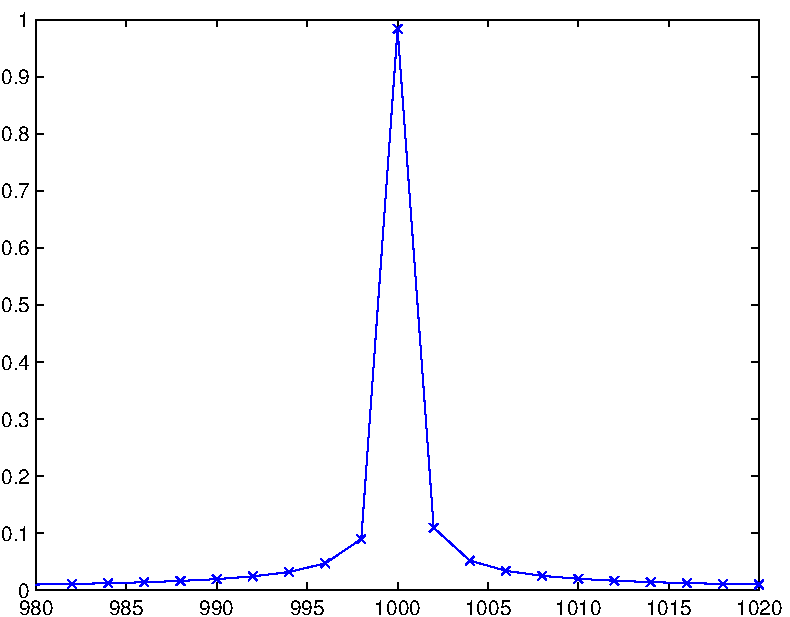
\includegraphics[width=0.7\textwidth]{qwtb_examples_published/qwtb_example_1_01.pdf}
\end{center}
\begin{par}
One can see it is not a coherent measurement. Therefore to get 'unknown' amplitude and frequency of the signal algorithm \lstinline{PSFE} can be used:
\end{par} \vspace{1em}
\begin{lstlisting}[style=mcode]
DO = qwtb('PSFE', DI);
f = DO.f.v
A = DO.A.v
\end{lstlisting}

        \begin{lstlisting}[style=output]
QWTB: no uncertainty calculation

f =

   1.0000e+03


A =

    1.0000

\end{lstlisting} \color{black}
    

\subsubsection*{Uncertainties}

\begin{par}
Uncertainties are added to the \lstinline{t} (time stamps) and \lstinline{y} (sampled data) structures.
\end{par} \vspace{1em}
\begin{lstlisting}[style=mcode]
DI.t.u = zeros(size(DI.t.v)) + 1e-5;
DI.y.u = zeros(size(DI.y.v)) + 1e-4;
\end{lstlisting}
\begin{par}
Calculations settings is created with Monte Carlo uncertainty calculation method, 1000 repeats and singlecore calculation.
\end{par} \vspace{1em}
\begin{lstlisting}[style=mcode]
CS.unc = 'mcm';
CS.mcm.repeats = 1000;
CS.mcm.method = 'singlecore';
\end{lstlisting}
\begin{par}
Run PSFE algorithm on input data \lstinline{DI} and with calculattion settings \lstinline{CS}.
\end{par} \vspace{1em}
\begin{lstlisting}[style=mcode]
DO = qwtb('PSFE',DI,CS);
\end{lstlisting}

        \begin{lstlisting}[style=output]
QWTB: default correlation matrix generated for quantity `t`
QWTB: quantity t was randomized by QWTB
QWTB: default correlation matrix generated for quantity `y`
QWTB: quantity y was randomized by QWTB
QWTB: general mcm uncertainty calculation
\end{lstlisting} \color{black}
    \begin{par}
Result is displayed as a histogram of calculated frequency.
\end{par} \vspace{1em}
\begin{lstlisting}[style=mcode]
figure; hist(DO.f.r,50);
\end{lstlisting}

\begin{center}
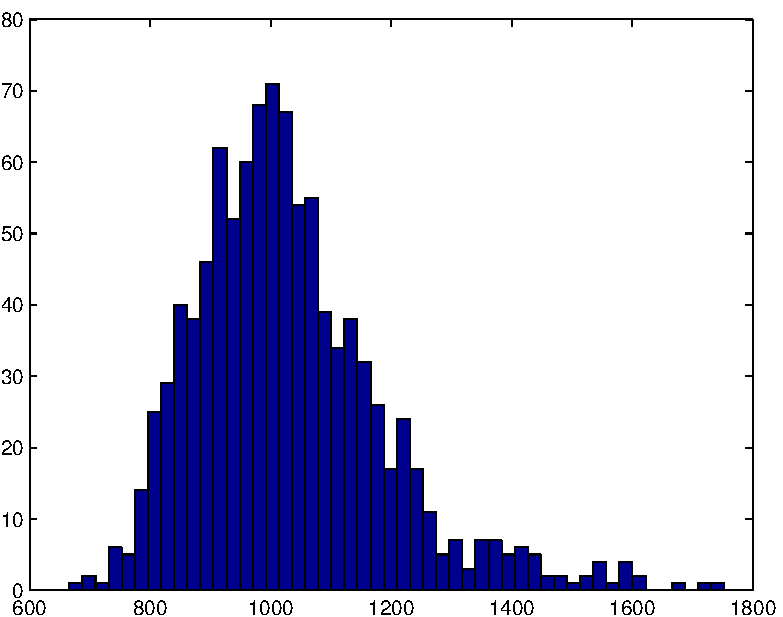
\includegraphics[width=0.7\textwidth]{qwtb_examples_published/qwtb_example_1_02.pdf}
\end{center}
\begin{par}
One can see the histogram is not Gaussian function. To get correct uncertainties, a shortest covariant interval has to be used.
\end{par} \vspace{1em}



%%% \end{document}
    


\chapter{Long example of QWTB use} %<<<1 ----------------------------------

% This LaTeX was auto-generated from an M-file by MATLAB.
% To make changes, update the M-file and republish this document.

%%% \documentclass{article}
%%% \usepackage{graphicx}
%%% \usepackage{color}

%%% \sloppy
%%% \definecolor{lightgray}{gray}{0.5}
\setlength{\parindent}{0pt}

%%% \begin{document}

    
    
\subsection*{Example of the QWTB use}

\begin{par}
Data are simulated, QWTB is used with different algorithms.
\end{par} \vspace{1em}

\subsubsection*{Contents}

\begin{itemize}
\setlength{\itemsep}{-1ex}
   \item Generate ideal data
   \item Apply three algorithms
   \item Compare results for ideal signal
   \item Noisy signal
   \item Compare results for noisy signal
   \item Non-coherent signal
   \item Compare results for non-coherent signal
   \item Harmonically distorted signal.
   \item Compare results for harmonically distorted signal.
   \item Harmonically distorted, noisy, non-coherent signal.
   \item Compare results for harmonically distorted, noisy, non-coherent signal.
\end{itemize}


\subsubsection*{Generate ideal data}

\begin{par}
Sample data are generated, representing 1 second of sine waveform of nominal frequency \lstinline{fnom} 1000 Hz, nominal amplitude \lstinline{Anom} 1 V and nominal phase \lstinline{phnom} 1 rad. Data are sampled at sampling frequency \lstinline{fsnom} 10 kHz, perfectly synchronized, no noise.
\end{par} \vspace{1em}
\begin{lstlisting}[style=mcode]
Anom = 1; fnom = 1000; phnom = 1; fsnom = 10e4;
timestamps = [0:1/fsnom:0.1-1/fsnom];
ideal_wave = Anom*sin(2*pi*fnom*timestamps + phnom);
\end{lstlisting}
\begin{par}
To use QWTB, data are put into two quantities: \lstinline{t} and \lstinline{y}. Both quantities are put into data in structure \lstinline{DI}.
\end{par} \vspace{1em}
\begin{lstlisting}[style=mcode]
DI = [];
DI.t.v = timestamps;
DI.y.v = ideal_wave;
\end{lstlisting}


\subsubsection*{Apply three algorithms}

\begin{par}
QWTB will be used to apply three algorithms to determine frequency and amplitude: \lstinline{SP-FFT}, \lstinline{PSFE} and \lstinline{FPNLSF}. Results are in data out structure \lstinline{DOxxx}. Algorithm \lstinline{FPNLSF} requires an estimate, select it to 0.1\% different from nominal frequency. \lstinline{SP-FFT} requires sampling frequency.
\end{par} \vspace{1em}
\begin{lstlisting}[style=mcode]
DI.fest.v = fnom.*1.001;
DI.fs.v = fsnom;
DOspfft = qwtb('SP-FFT', DI);
DOpsfe = qwtb('PSFE', DI);
DOfpnlsf = qwtb('FPNLSF', DI);
\end{lstlisting}

        \begin{lstlisting}[style=output]
QWTB: no uncertainty calculation
QWTB: no uncertainty calculation
QWTB: PSFE wrapper: sampling time was calculated from sampling frequency
QWTB: no uncertainty calculation
Fitting started

Local minimum found.

Optimization completed because the size of the gradient is less than
the default value of the function tolerance.



Fitting finished
\end{lstlisting} \color{black}
    

\subsubsection*{Compare results for ideal signal}

\begin{par}
Calculate relative errors in ppm for all algorithm to know which one is best. \lstinline{SP-FFT} returns whole spectrum, so only the largest amplitude peak is interesting. One can see for the ideal case all errors are very small.
\end{par} \vspace{1em}
\begin{lstlisting}[style=mcode]
disp('SP-FFT errors (ppm):')
[tmp, ind] = max(DOspfft.A.v);
ferr  = (DOspfft.f.v(ind) - fnom)/fnom .* 1e6
Aerr  = (DOspfft.A.v(ind) - Anom)/Anom .* 1e6
pherr = (DOspfft.ph.v(ind) - phnom)/phnom .* 1e6

disp('PSFE errors (ppm):')
ferr  = (DOpsfe.f.v - fnom)/fnom .* 1e6
Aerr  = (DOpsfe.A.v - Anom)/Anom .* 1e6
pherr = (DOpsfe.ph.v - phnom)/phnom .* 1e6

disp('FPNLSF errors (ppm):')
ferr  = (DOfpnlsf.f.v - fnom)/fnom .* 1e6
Aerr  = (DOfpnlsf.A.v - Anom)/Anom .* 1e6
pherr = (DOfpnlsf.ph.v - phnom)/phnom .* 1e6
\end{lstlisting}

        \begin{lstlisting}[style=output]
SP-FFT errors (ppm):

ferr =

     0


Aerr =

     0


pherr =

  -4.2920e+05

PSFE errors (ppm):

ferr =

  -2.2737e-10


Aerr =

   4.8850e-09


pherr =

   2.3093e-08

FPNLSF errors (ppm):

ferr =

  -3.4106e-10


Aerr =

  -4.0512e-07


pherr =

   1.8208e-08

\end{lstlisting} \color{black}
    

\subsubsection*{Noisy signal}

\begin{par}
To simulate real measurement, noise is added with normal distribution and standard deviation \lstinline{sigma} of 100 microvolt. Algorithms are again applied.
\end{par} \vspace{1em}
\begin{lstlisting}[style=mcode]
sigma = 100e-6;
DI.y.v = ideal_wave + 100e-6.*randn(size(ideal_wave));
DOspfft = qwtb('SP-FFT', DI);
DOpsfe = qwtb('PSFE', DI);
DOfpnlsf = qwtb('FPNLSF', DI);
\end{lstlisting}

        \begin{lstlisting}[style=output]
QWTB: no uncertainty calculation
QWTB: no uncertainty calculation
QWTB: PSFE wrapper: sampling time was calculated from sampling frequency
QWTB: no uncertainty calculation
Fitting started

Local minimum found.

Optimization completed because the size of the gradient is less than
the default value of the function tolerance.



Fitting finished
\end{lstlisting} \color{black}
    

\subsubsection*{Compare results for noisy signal}

\begin{par}
Again relative errors are compared. One can see amplitude and phase errors increased to several ppm, however frequency is still determined quite good by all three algorithms. FFT is not affected by noise at all.
\end{par} \vspace{1em}
\begin{lstlisting}[style=mcode]
disp('SP-FFT errors (ppm):')
[tmp, ind] = max(DOspfft.A.v);
ferr  = (DOspfft.f.v(ind) - fnom)/fnom .* 1e6
Aerr  = (DOspfft.A.v(ind) - Anom)/Anom .* 1e6
pherr = (DOspfft.ph.v(ind) - phnom)/phnom .* 1e6

disp('PSFE errors:')
ferr  = (DOpsfe.f.v - fnom)/fnom .* 1e6
Aerr  = (DOpsfe.A.v - Anom)/Anom .* 1e6
pherr = (DOpsfe.ph.v - phnom)/phnom .* 1e6

disp('FPNLSF errors:')
ferr  = (DOfpnlsf.f.v - fnom)/fnom .* 1e6
Aerr  = (DOfpnlsf.A.v - Anom)/Anom .* 1e6
pherr = (DOfpnlsf.ph.v - phnom)/phnom .* 1e6
\end{lstlisting}

        \begin{lstlisting}[style=output]
SP-FFT errors (ppm):

ferr =

     0


Aerr =

   -0.6603


pherr =

  -4.2920e+05

PSFE errors:

ferr =

    0.0010


Aerr =

   -0.6318


pherr =

   -1.0933

FPNLSF errors:

ferr =

   -0.0011


Aerr =

   -0.6601


pherr =

   -0.3809

\end{lstlisting} \color{black}
    

\subsubsection*{Non-coherent signal}

\begin{par}
In real measurement coherent measurement does not exist. So in next test the frequency of the signal differs by 20 ppm:
\end{par} \vspace{1em}
\begin{lstlisting}[style=mcode]
fnc = fnom*(1 + 20e-6);
noncoh_wave = Anom*sin(2*pi*fnc*timestamps + phnom);
DI.y.v = noncoh_wave;
DOspfft = qwtb('SP-FFT', DI);
DOpsfe = qwtb('PSFE', DI);
DOfpnlsf = qwtb('FPNLSF', DI);
\end{lstlisting}

        \begin{lstlisting}[style=output]
QWTB: no uncertainty calculation
QWTB: no uncertainty calculation
QWTB: PSFE wrapper: sampling time was calculated from sampling frequency
QWTB: no uncertainty calculation
Fitting started

Local minimum found.

Optimization completed because the size of the gradient is less than
the default value of the function tolerance.



Fitting finished
\end{lstlisting} \color{black}
    

\subsubsection*{Compare results for non-coherent signal}

\begin{par}
Comparison of relative errors. Results of \lstinline{PSFE} or \lstinline{FPNLSF} are correct, however FFT is affected by non-coherent signal considerably.
\end{par} \vspace{1em}
\begin{lstlisting}[style=mcode]
disp('SP-FFT errors (ppm):')
[tmp, ind] = max(DOspfft.A.v);
ferr  = (DOspfft.f.v(ind) - fnc)/fnc .* 1e6
Aerr  = (DOspfft.A.v(ind) - Anom)/Anom .* 1e6
pherr = (DOspfft.ph.v(ind) - phnom)/phnom .* 1e6

disp('PSFE errors:')
ferr  = (DOpsfe.f.v - fnc)/fnc .* 1e6
Aerr  = (DOpsfe.A.v - Anom)/Anom .* 1e6
pherr = (DOpsfe.ph.v - phnom)/phnom .* 1e6

disp('FPNLSF errors:')
ferr  = (DOfpnlsf.f.v - fnc)/fnc .* 1e6
Aerr  = (DOfpnlsf.A.v - Anom)/Anom .* 1e6
pherr = (DOfpnlsf.ph.v - phnom)/phnom .* 1e6
\end{lstlisting}

        \begin{lstlisting}[style=output]
SP-FFT errors (ppm):

ferr =

  -19.9996


Aerr =

   -2.8780


pherr =

  -4.3550e+05

PSFE errors:

ferr =

  -1.1368e-10


Aerr =

   3.8924e-07


pherr =

   3.3073e-04

FPNLSF errors:

ferr =

  -1.1368e-10


Aerr =

  -3.2940e-07


pherr =

   2.6867e-08

\end{lstlisting} \color{black}
    

\subsubsection*{Harmonically distorted signal.}

\begin{par}
In other cases a harmonic distortion can appear. Suppose a signal with second order harmonic of 10\% amplitude as the main signal.
\end{par} \vspace{1em}
\begin{lstlisting}[style=mcode]
hadist_wave = Anom*sin(2*pi*fnom*timestamps + phnom) + 0.1*Anom*sin(2*pi*fnom*2*timestamps + 2);
DI.y.v = hadist_wave;
DOspfft = qwtb('SP-FFT', DI);
DOpsfe = qwtb('PSFE', DI);
DOfpnlsf = qwtb('FPNLSF', DI);
\end{lstlisting}

        \begin{lstlisting}[style=output]
QWTB: no uncertainty calculation
QWTB: no uncertainty calculation
QWTB: PSFE wrapper: sampling time was calculated from sampling frequency
QWTB: no uncertainty calculation
Fitting started

Local minimum found.

Optimization completed because the size of the gradient is less than
the default value of the function tolerance.



Fitting finished
\end{lstlisting} \color{black}
    

\subsubsection*{Compare results for harmonically distorted signal.}

\begin{par}
Comparison of relative errors. \lstinline{SP-FFT} or \lstinline{PSFE} are not affected by harmonic distortion, however \lstinline{FPNLSF} is thus is not suitable for such signal.
\end{par} \vspace{1em}
\begin{lstlisting}[style=mcode]
disp('SP-FFT errors (ppm):')
[tmp, ind] = max(DOspfft.A.v);
ferr  = (DOspfft.f.v(ind) - fnom)/fnom .* 1e6
Aerr  = (DOspfft.A.v(ind) - Anom)/Anom .* 1e6
pherr = (DOspfft.ph.v(ind) - phnom)/phnom .* 1e6

disp('PSFE errors:')
ferr  = (DOpsfe.f.v - fnom)/fnom .* 1e6
Aerr  = (DOpsfe.A.v - Anom)/Anom .* 1e6
pherr = (DOpsfe.ph.v - phnom)/phnom .* 1e6

disp('FPNLSF errors:')
ferr  = (DOfpnlsf.f.v - fnom)/fnom .* 1e6
Aerr  = (DOfpnlsf.A.v - Anom)/Anom .* 1e6
pherr = (DOfpnlsf.ph.v - phnom)/phnom .* 1e6
\end{lstlisting}

        \begin{lstlisting}[style=output]
SP-FFT errors (ppm):

ferr =

     0


Aerr =

     0


pherr =

  -4.2920e+05

PSFE errors:

ferr =

  -2.2737e-10


Aerr =

   6.7212e-04


pherr =

    0.5311

FPNLSF errors:

ferr =

   -0.7356


Aerr =

    0.1407


pherr =

  231.4553

\end{lstlisting} \color{black}
    

\subsubsection*{Harmonically distorted, noisy, non-coherent signal.}

\begin{par}
In final test all distortions are put in a waveform and results are compared.
\end{par} \vspace{1em}
\begin{lstlisting}[style=mcode]
err_wave = Anom*sin(2*pi*fnc*timestamps + phnom) + 0.1*Anom*sin(2*pi*fnc*2*timestamps + 2) + 100e-6.*randn(size(ideal_wave));
DI.y.v = err_wave;
DOspfft = qwtb('SP-FFT', DI);
DOpsfe = qwtb('PSFE', DI);
DOfpnlsf = qwtb('FPNLSF', DI);
\end{lstlisting}

        \begin{lstlisting}[style=output]
QWTB: no uncertainty calculation
QWTB: no uncertainty calculation
QWTB: PSFE wrapper: sampling time was calculated from sampling frequency
QWTB: no uncertainty calculation
Fitting started

Local minimum found.

Optimization completed because the size of the gradient is less than
the default value of the function tolerance.



Fitting finished
\end{lstlisting} \color{black}
    

\subsubsection*{Compare results for harmonically distorted, noisy, non-coherent signal.}

\begin{lstlisting}[style=mcode]
disp('SP-FFT errors (ppm):')
[tmp, ind] = max(DOspfft.A.v);
ferr  = (DOspfft.f.v(ind) - fnc)/fnc .* 1e6
Aerr  = (DOspfft.A.v(ind) - Anom)/Anom .* 1e6
pherr = (DOspfft.ph.v(ind) - phnom)/phnom .* 1e6

disp('PSFE errors:')
ferr  = (DOpsfe.f.v - fnc)/fnc .* 1e6
Aerr  = (DOpsfe.A.v - Anom)/Anom .* 1e6
pherr = (DOpsfe.ph.v - phnom)/phnom .* 1e6

disp('FPNLSF errors:')
ferr  = (DOfpnlsf.f.v - fnc)/fnc .* 1e6
Aerr  = (DOfpnlsf.A.v - Anom)/Anom .* 1e6
pherr = (DOfpnlsf.ph.v - phnom)/phnom .* 1e6
\end{lstlisting}

        \begin{lstlisting}[style=output]
SP-FFT errors (ppm):

ferr =

  -19.9996


Aerr =

    1.1501


pherr =

  -4.3550e+05

PSFE errors:

ferr =

   -0.0072


Aerr =

    4.1189


pherr =

    4.6464

FPNLSF errors:

ferr =

   -0.7241


Aerr =

    3.6943


pherr =

  229.3720

\end{lstlisting} \color{black}
    


%%% \end{document}
    


\chapter{INL -- Integral Non-Linearity of ADC} %<<<1 ------------------------------
\def\infosection{Info file data}
\def\examplesection{Example}
% included files are automatically generated by info_all_algs.m script and by Matlab publish
% function and converted by bash script betterpublish.
\section*{\infosection} %<<<2 -------------------
\begin{tightdesc}
\item [\textsf{.id}] --- INL
\item [\textsf{.name}] --- Integral Non-Linearity of ADC
\item [\textsf{.desc}] --- Calculates Integral Non-Linearity of an ADC. ADC has to sample sinewave, ADC codes are required.
\item [\textsf{.citation}] --- Virosztek, T., Pálfi V., Renczes B., Kollár I., Balogh L., Sárhegyi A., Márkus J., Bilau Z. T., ADCTest project site: \url{http://www.mit.bme.hu/projects/adctest} 2000-2014
\item [\textsf{.remarks}] --- Based on the ADCTest Toolbox v4.3, November 25, 2014.
\item [\textsf{.license}] --- UNKNOWN
\item [\textsf{.requires}] \rule{0em}{0em}
\begin{tightdesc}
\item [\textsf{t}] --- time series of sampled data
\item [\textsf{codes}] --- Sampled values represented as ADC codes (not converted to voltage)
\end{tightdesc}
\item [\textsf{.returns}] \rule{0em}{0em}
\begin{tightdesc}
\item [\textsf{INL}] --- INL
\end{tightdesc}
\item [\textsf{.providesGUF}] --- no
\item [\textsf{.providesMCM}] ---  no
\end{tightdesc}

\section*{\examplesection} %<<<2 ------------------------

% This LaTeX was auto-generated from an M-file by MATLAB.
% To make changes, update the M-file and republish this document.

%%% \documentclass{article}
%%% \usepackage{graphicx}
%%% \usepackage{color}

%%% \sloppy
%%% \definecolor{lightgray}{gray}{0.5}
\setlength{\parindent}{0pt}

%%% \begin{document}

    
    
\subsection*{Integral Non Linearity of ADC}

\begin{par}
Example for algorithm INL
\end{par} \vspace{1em}
\begin{par}
INL is an algorithm for estimating Integral Non-Linearity of an ADC. ADC has to sample sinewave, ADC codes are required.
\end{par} \vspace{1em}
\begin{par}
See also 'Virosztek, T., Pálfi V., Renczes B., Kollár I., Balogh L., Sárhegyi A., Márkus J., Bilau Z. T., ADCTest project site: \url{http://www.mit.bme.hu/projects/adctest} 2000-2014';
\end{par} \vspace{1em}

\subsubsection*{Contents}

\begin{itemize}
\setlength{\itemsep}{-1ex}
   \item Generate sample data
   \item Call algorithm
\end{itemize}


\subsubsection*{Generate sample data}

\begin{par}
Suppose a sine wave of nominal frequency 10 Hz and nominal amplitude 1 V is sampled by ADC with bit resolution of 4. First quantities \lstinline{t} with time of samples and quantity \lstinline{bits} with number of bits are prepared and put into input data structure \lstinline{DI}.
\end{par} \vspace{1em}
\begin{lstlisting}[style=mcode]
DI = [];
DI.t.v=[0:1/1e4:1-1/1e4];
DI.bits.v = 4;
\end{lstlisting}
\begin{par}
Waveform is constructed.
\end{par} \vspace{1em}
\begin{lstlisting}[style=mcode]
Anom = 1; fnom = 2; phnom = 0;
wvfrm = Anom*sin(2*pi*fnom*DI.t.v + phnom);
\end{lstlisting}
\begin{par}
Next code values are calculated. It is simulated by quantization and scaling of the sampled waveform. In real measurement code values can be obtained directly from the ADC. Suppose ADC range is -1..1.
\end{par} \vspace{1em}
\begin{lstlisting}[style=mcode]
codes = wvfrm;
rmin = -1; rmax = 1;
levels = 2.^DI.bits.v - 1;
codes(codes<rmin) = rmin;
codes(codes>rmax) = rmax;
codes = round((codes-rmin)./2.*levels);
\end{lstlisting}
\begin{par}
Now lets introduce ADC error. Instead of generating code 2 ADC erroneously generates code 3 and instead of 10 it generates 11.
\end{par} \vspace{1em}
\begin{lstlisting}[style=mcode]
codes(codes==2) = 3;
codes(codes==10) = 11;
codes = codes + min(codes);
\end{lstlisting}
\begin{par}
Create quantity \lstinline{codes} and plot a figure with sampled sine wave and codes.
\end{par} \vspace{1em}
\begin{lstlisting}[style=mcode]
DI.codes.v = codes;
figure
%plot(t, (y+1).*1/2.*levels, t, codes);
hold on
stairs(DI.t.v, codes);
wvfrm = (wvfrm + Anom).*levels./2;
plot(DI.t.v, wvfrm, '-r');
xlabel('t (s)')
ylabel('Codes / Voltage (scaled)');
legend('Codes generated by ADC','Original waveform scaled to match codes');
hold off
\end{lstlisting}

\begin{center}
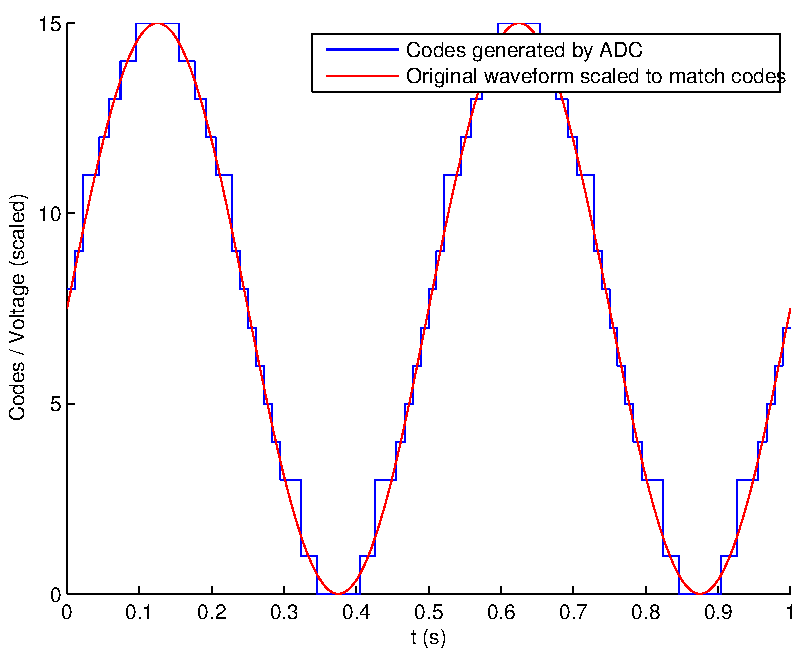
\includegraphics[width=0.7\textwidth]{alg_examples_published/INL_alg_example_01.pdf}
\end{center}


\subsubsection*{Call algorithm}

\begin{par}
Apply INL algorithm to the input data \lstinline{DI}.
\end{par} \vspace{1em}
\begin{lstlisting}[style=mcode]
DO = qwtb('INL', DI);
\end{lstlisting}

        \begin{lstlisting}[style=output]
QWTB: no uncertainty calculation
\end{lstlisting} \color{black}
    \begin{par}
Plot results of integral non-linearity. One can clearly observe defects on codes 3 and 11.
\end{par} \vspace{1em}
\begin{lstlisting}[style=mcode]
figure
plot(DO.INL.v, '-x');
xlabel('Code value')
ylabel('INL')
\end{lstlisting}

\begin{center}
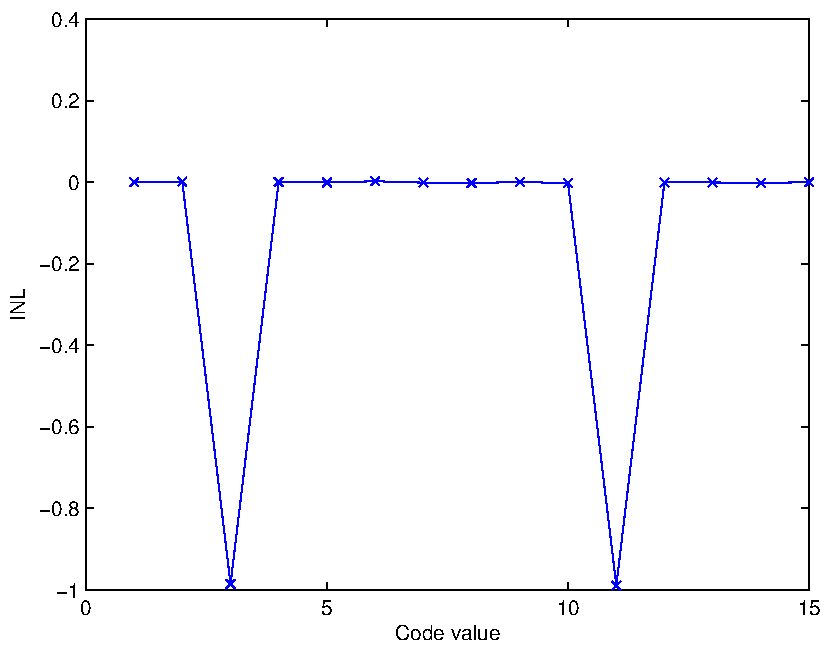
\includegraphics[width=0.7\textwidth]{alg_examples_published/INL_alg_example_02.pdf}
\end{center}



%%% \end{document}
    


\chapter{PSFE -- Phase Sensitive Frequency Estimator} %<<<1 ------------------------------
% included files are automatically generated by info_all_algs.m script and by Matlab publish
% function and converted by bash script betterpublish.
\section*{\infosection} %<<<2 -------------------
\begin{tightdesc}
\item [Id:] PSFE
\item [Name:] Phase Sensitive Frequency Estimator
\item [Description:] An algorithm for estimating the frequency, amplitude, and phase of the fundamental component in harmonically distorted waveforms. The algorithm minimizes the phase difference between the sine model and the sampled waveform by effectively minimizing the influence of the harmonic components. It uses a three-parameter sine-fitting algorithm for all phase calculations. The resulting estimates show up to two orders of magnitude smaller sensitivity to harmonic distortions than the results of the four-parameter sine fitting algorithm.
\item [Citation:] Lapuh, R., "Estimating the Fundamental Component of Harmonically Distorted Signals From Noncoherently Sampled Data," Instrumentation and Measurement, IEEE Transactions on , vol.64, no.6, pp.1419,1424, June 2015, doi: 10.1109/TIM.2015.2401211, URL: \url{http://ieeexplore.ieee.org/stamp/stamp.jsp?tp=\&arnumber=7061456\&isnumber=7104190}
\item [Remarks:] If sampling time |Ts| is not supplied, wrapper will calculate |Ts| from sampling frequency |fs| or if not supplied, mean of differences of time series |t| is used to calculate |Ts|.
\item [License:] MIT License
\item [Provides GUF:] no
\item [Provides MCM:] no
\item [Input Quantities] \rule{0em}{0em}
    \begin{tightdesc}
    \item [Required:] 
        \textsf{Ts} or \textsf{fs} or \textsf{t},\enspace \textsf{y}
    \item [Descriptions:] \rule{0em}{0em}
        \begin{tightdesc}
            \item[\textsf{Ts}] -- Sampling time
            \item[\textsf{fs}] -- Sampling frequency
            \item[\textsf{t}] -- Time series
            \item[\textsf{y}] -- Sampled values
        \end{tightdesc}
    \end{tightdesc}
\item [Output Quantities:] \rule{0em}{0em}
    \begin{tightdesc}
        \item[\textsf{A}] -- Amplitude of main signal component
        \item[\textsf{f}] -- Frequency of main signal component
        \item[\textsf{ph}] -- Phase of main signal component
    \end{tightdesc}
\end{tightdesc}

\section*{\examplesection} %<<<2 ------------------------

% This LaTeX was auto-generated from an M-file by MATLAB.
% To make changes, update the M-file and republish this document.

%%% \documentclass{article}
%%% \usepackage{graphicx}
%%% \usepackage{color}

%%% \sloppy
%%% \definecolor{lightgray}{gray}{0.5}
\setlength{\parindent}{0pt}

%%% \begin{document}

    
    
\subsection*{Phase Sensitive Frequency Estimator}

\begin{par}
Example for algorithm PSFE.
\end{par} \vspace{1em}
\begin{par}
PSFE is an algorithm for estimating the frequency, amplitude, and phase of the fundamental component in harmonically distorted waveforms. The algorithm minimizes the phase difference between the sine model and the sampled waveform by effectively minimizing the influence of the harmonic components. It uses a three-parameter sine-fitting algorithm for all phase calculations. The resulting estimates show up to two orders of magnitude smaller sensitivity to harmonic distortions than the results of the four-parameter sine fitting algorithm.
\end{par} \vspace{1em}
\begin{par}
See also Lapuh, R., "Estimating the Fundamental Component of Harmonically Distorted Signals From Noncoherently Sampled Data," Instrumentation and Measurement, IEEE Transactions on , vol.64, no.6, pp.1419,1424, June 2015, doi: 10.1109/TIM.2015.2401211, URL: \url{http://ieeexplore.ieee.org/stamp/stamp.jsp?tp=&arnumber=7061456&isnumber=7104190}'
\end{par} \vspace{1em}

\subsubsection*{Contents}

\begin{itemize}
\setlength{\itemsep}{-1ex}
   \item Generate sample data
   \item Call algorithm
   \item Display results
\end{itemize}


\subsubsection*{Generate sample data}

\begin{par}
Two quantities are prepared: \lstinline{t} and \lstinline{y}, representing 1 second of sinus waveform of nominal frequency 100 Hz, nominal amplitude 1 V and nominal phase 1 rad, sampled at sampling frequency 10 kHz.
\end{par} \vspace{1em}
\begin{lstlisting}[style=mcode]
DI = [];
Anom = 1; fnom = 100; phnom = 1;
DI.t.v = [0:1/1e4:1-1/1e4];
DI.y.v = Anom*sin(2*pi*fnom*DI.t.v + phnom);
\end{lstlisting}
\begin{par}
Add noise:
\end{par} \vspace{1em}
\begin{lstlisting}[style=mcode]
DI.y.v = DI.y.v + normrnd(0, 1e-3, size(DI.y.v));
\end{lstlisting}


\subsubsection*{Call algorithm}

\begin{par}
Use QWTB to apply algorithm \lstinline{PSFE} to data \lstinline{DI}.
\end{par} \vspace{1em}
\begin{lstlisting}[style=mcode]
DO = qwtb('PSFE', DI);
\end{lstlisting}

        \begin{lstlisting}[style=output]
QWTB: no uncertainty calculation
\end{lstlisting} \color{black}
    

\subsubsection*{Display results}

\begin{par}
Results is the amplitude, frequency and phase of sampled waveform.
\end{par} \vspace{1em}
\begin{lstlisting}[style=mcode]
f = DO.f.v
A = DO.A.v
ph = DO.ph.v
\end{lstlisting}

        \begin{lstlisting}[style=output]

f =

  100.0000


A =

    1.0000


ph =

    1.0000

\end{lstlisting} \color{black}
    \begin{par}
Errors of estimation in parts per milion:
\end{par} \vspace{1em}
\begin{lstlisting}[style=mcode]
ferrppm = (DO.f.v - fnom)/fnom .* 1e6
Aerrppm = (DO.A.v - Anom)/Anom .* 1e6
pherrppm = (DO.ph.v - phnom)/phnom .* 1e6
\end{lstlisting}

        \begin{lstlisting}[style=output]

ferrppm =

    0.1113


Aerrppm =

    4.3774


pherrppm =

  -13.7952

\end{lstlisting} \color{black}
    


%%% \end{document}
    


\chapter{FPSWF -- Four Parameter Sine Wave Fitting} %<<<1 ------------------------------
% included files are automatically generated by info_all_algs.m script and by Matlab publish
% function and converted by bash script betterpublish.
\section*{\infosection} %<<<2 -------------------
\begin{tightdesc}
\item [\textsf{.id}] --- FPSWF
\item [\textsf{.name}] --- Four Parameter Sine Wave Fit
\item [\textsf{.desc}] --- Fits a sine wave to the recorded data by means of least squares fitting using 4 parameter (frequency, amplitude, phase and offset) model. An estimate of signal frequency is required. Due to non-linear characteristic, converge is not always achieved. When run in Matlab, function `lsqnonlin` in Optimization toolbox is used. When run in GNU Octave, function `leasqr` in GNU Octave Forge package optim is used.
\item [\textsf{.citation}] --- 
\item [\textsf{.remarks}] --- Algorithm works essentially only for simple sine wave. Algorithm is very sensitive to distortion. Algorithm requires good estimate of signal frequency.
\item [\textsf{.license}] --- MIT License
\item [\textsf{.requires}] \rule{0em}{0em}
\begin{tightdesc}
\item [\textsf{t}] --- Time series of sampled data
\item [\textsf{y}] --- Sampled values
\item [\textsf{fest}] --- Estimate of signal frequency
\end{tightdesc}
\item [\textsf{.returns}] \rule{0em}{0em}
\begin{tightdesc}
\item [\textsf{f}] --- Frequency of main signal component
\item [\textsf{A}] --- Amplitude of main signal component
\item [\textsf{ph}] --- Phase of main signal component
\item [\textsf{O}] --- Offset of signal
\end{tightdesc}
\item [\textsf{.providesGUF}] --- no
\item [\textsf{.providesMCM}] ---  no
\end{tightdesc}

\section*{\examplesection} %<<<2 ------------------------

% This LaTeX was auto-generated from an M-file by MATLAB.
% To make changes, update the M-file and republish this document.

%%% \documentclass{article}
%%% \usepackage{graphicx}
%%% \usepackage{color}

%%% \sloppy
%%% \definecolor{lightgray}{gray}{0.5}
\setlength{\parindent}{0pt}

%%% \begin{document}

    
    
\subsection*{Four parameter sine wave fitting}

\begin{par}
Example for algorithm FPSWF.
\end{par} \vspace{1em}
\begin{par}
FPSWF is an algorithm for estimating the frequency, amplitude, and phase of the sine waveform. The algorithm use least squares method. Algorithm requires good estimate of frequency.
\end{par} \vspace{1em}

\subsubsection*{Contents}

\begin{itemize}
\setlength{\itemsep}{-1ex}
   \item Generate sample data
   \item Call algorithm
   \item Display results
\end{itemize}


\subsubsection*{Generate sample data}

\begin{par}
Two quantities are prepared: \lstinline{t} and \lstinline{y}, representing 1 second of sinus waveform of nominal frequency 1 kHz, nominal amplitude 1 V, nominal phase 1 rad and offset 1 V sampled at sampling frequency 10 kHz.
\end{par} \vspace{1em}
\begin{lstlisting}[style=mcode]
DI = [];
Anom = 2; fnom = 100; phnom = 1; Onom = 0.2;
DI.t.v = [0:1/1e4:1-1/1e4];
DI.y.v = Anom*sin(2*pi*fnom*DI.t.v + phnom) + Onom;
\end{lstlisting}
\begin{par}
Lets make an estimate of frequency 0.2 percent higher than nominal value:
\end{par} \vspace{1em}
\begin{lstlisting}[style=mcode]
DI.f.v = 100.2;
\end{lstlisting}


\subsubsection*{Call algorithm}

\begin{par}
Use QWTB to apply algorithm \lstinline{FPSWF} to data \lstinline{DI}.
\end{par} \vspace{1em}
\begin{lstlisting}[style=mcode]
CS.verbose = 1;
DO = qwtb('FPSWF', DI, CS);
\end{lstlisting}

        \begin{lstlisting}[style=output]
QWTB: no uncertainty calculation
Fitting started

Local minimum found.

Optimization completed because the size of the gradient is less than
the default value of the function tolerance.



Fitting finished
\end{lstlisting} \color{black}
    

\subsubsection*{Display results}

\begin{par}
Results is the amplitude, frequency and phase of sampled waveform.
\end{par} \vspace{1em}
\begin{lstlisting}[style=mcode]
A = DO.A.v
f = DO.f.v
ph = DO.ph.v
O = DO.O.v
\end{lstlisting}

        \begin{lstlisting}[style=output]

A =

    2.0000


f =

  100.0000


ph =

    1.0000


O =

   -0.2000

\end{lstlisting} \color{black}
    \begin{par}
Errors of estimation in parts per milion:
\end{par} \vspace{1em}
\begin{lstlisting}[style=mcode]
Aerrppm = (DO.A.v - Anom)/Anom .* 1e6
ferrppm = (DO.f.v - fnom)/fnom .* 1e6
pherrppm = (DO.ph.v - phnom)/phnom .* 1e6
Oerrppm = (DO.O.v - Onom)/Onom .* 1e6
\end{lstlisting}

        \begin{lstlisting}[style=output]

Aerrppm =

   4.8894e-07


ferrppm =

  -1.4211e-10


pherrppm =

   1.7542e-08


Oerrppm =

  -2.0000e+06

\end{lstlisting} \color{black}
    


%%% \end{document}
    


\chapter{SP-FFT -- Spectrum by means of Fast Fourier Transform} %<<<1 ------------------------------
% included files are automatically generated by info_all_algs.m script and by Matlab publish
% function and converted by bash script betterpublish.
\section*{\infosection} %<<<2 -------------------
\begin{tightdesc}
\item [\textsf{.id}] --- SP-FFT
\item [\textsf{.name}] --- Spectrum by means of Fast Fourier Transform
\item [\textsf{.desc}] --- Calculates frequency and phase spectrum by means of Fast Fourier Transform algorithm. Result is normalized.
\item [\textsf{.citation}] --- 
\item [\textsf{.remarks}] --- 
\item [\textsf{.license}] --- MIT License
\item [\textsf{.requires}] \rule{0em}{0em}
\begin{tightdesc}
\item [\textsf{y}] --- Sampled values
\item [\textsf{fs}] --- Sampling frequency
\end{tightdesc}
\item [\textsf{.returns}] \rule{0em}{0em}
\begin{tightdesc}
\item [\textsf{f}] --- Frequency series
\item [\textsf{A}] --- Amplitude series
\item [\textsf{ph}] --- Phase series
\end{tightdesc}
\item [\textsf{.providesGUF}] --- no
\item [\textsf{.providesMCM}] ---  no
\end{tightdesc}

\section*{\examplesection} %<<<2 ------------------------

% This LaTeX was auto-generated from an M-file by MATLAB.
% To make changes, update the M-file and republish this document.

%%% \documentclass{article}
%%% \usepackage{graphicx}
%%% \usepackage{color}

%%% \sloppy
%%% \definecolor{lightgray}{gray}{0.5}
\setlength{\parindent}{0pt}

%%% \begin{document}

    
    
\subsection*{Signal Spectrum by means of Fast fourier transform}

\begin{par}
Example for algorithm SP-FFT.
\end{par} \vspace{1em}
\begin{par}
Calculates frequency and phase spectrum by means of Fast Fourier Transform algorithm. Result is normalized.
\end{par} \vspace{1em}

\subsubsection*{Contents}

\begin{itemize}
\setlength{\itemsep}{-1ex}
   \item Generate sample data
   \item Call algorithm
   \item Display results
\end{itemize}


\subsubsection*{Generate sample data}

\begin{par}
Two quantities are prepared: \lstinline{y} and \lstinline{fs}, representing 1 second of signal containing 5 harmonic components and one inter-harmonic component. Main signal component has nominal frequency 1 kHz, nominal amplitude 2 V, nominal phase 1 rad and offset 1 V sampled at sampling frequency 10 kHz.
\end{par} \vspace{1em}
\begin{lstlisting}[style=mcode]
DI = [];
fsnom = 1e4; Anom = 2; fnom = 100; phnom = 1; Onom = 0.2;
t = [0:1/fsnom:1-1/fsnom];
DI.y.v = Anom*sin(2*pi*fnom*t + phnom);
for i = 2:45
        DI.y.v = DI.y.v + Anom./i*sin(2*pi*fnom*i*t + phnom + i - 1);
end
DI.y.v = DI.y.v + 1*sin(2*pi*fnom*1.456*t + phnom);
DI.fs.v = fsnom;
\end{lstlisting}


\subsubsection*{Call algorithm}

\begin{par}
Use QWTB to apply algorithm \lstinline{SP-FFT} to data \lstinline{DI}.
\end{par} \vspace{1em}
\begin{lstlisting}[style=mcode]
DO = qwtb('SP-FFT', DI);
\end{lstlisting}

        \begin{lstlisting}[style=output]
QWTB: no uncertainty calculation
\end{lstlisting} \color{black}
    

\subsubsection*{Display results}

\begin{par}
Results is the amplitude and phase spectrum.
\end{par} \vspace{1em}
\begin{lstlisting}[style=mcode]
figure
plot(DO.f.v, DO.A.v, '-x')
xlabel('f (Hz)'); ylabel('A (V)'); title('Amplitude spectrum of the signal');
figure
plot(DO.f.v, DO.ph.v, '-x')
xlabel('f (Hz)'); ylabel('phase (rad)'); title('Phase spectrum of the signal');
\end{lstlisting}

\begin{center}
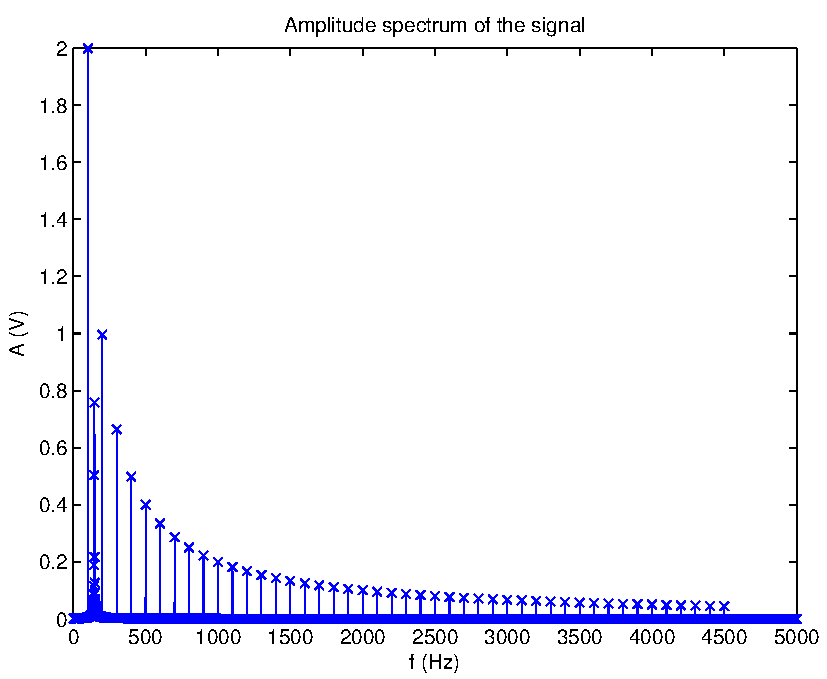
\includegraphics[width=0.7\textwidth]{algs_examples_published/SP-FFT_alg_example_01.pdf}
\end{center}

\begin{center}
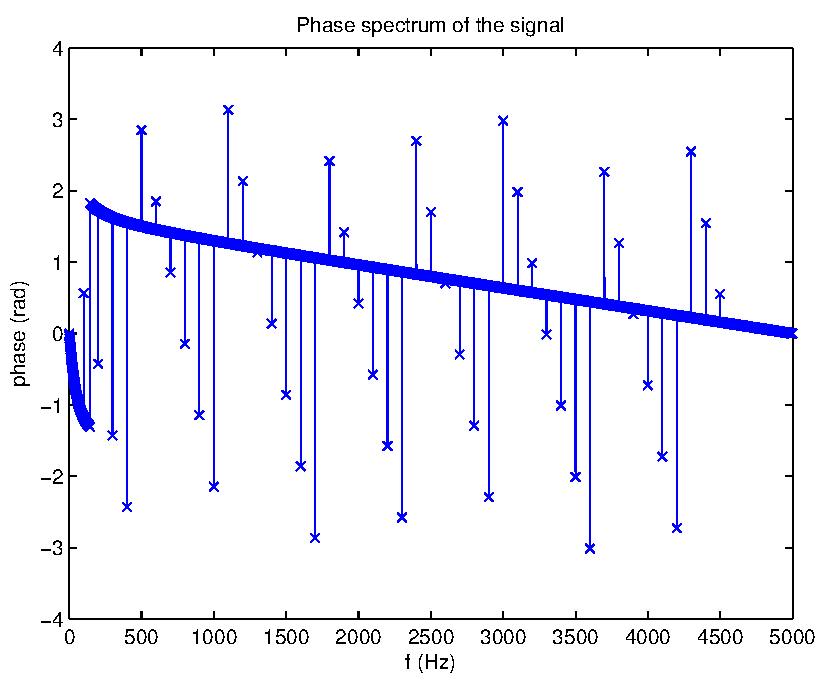
\includegraphics[width=0.7\textwidth]{algs_examples_published/SP-FFT_alg_example_02.pdf}
\end{center}



%%% \end{document}
    




% from DELIVERABLE %<<<1 
% \section{Introduction} %<<<2 ------------------------------
% The following report is on the plan for software in preparation. The software should serve as
% a~\Tb for evaluation of digital or quantum generators errors. The goal is:
% 
% {\small \it
% \dots is to develop a software toolbox for the evaluation of quantum source and metrology
% grade ADCs errors and their related measurement uncertainties. \dots It will be prepared to serve as
% an uncertainty calculator for actual sampled data, as well as a stand-alone analysis tool to study
% errors and related uncertainties as a function of various signal and sampling parameters (e.g.
% signal frequency, noise level, signal distortions, timing errors). Multiple uncertainty estimation
% methods will be used, such as GUM Framework and Monte Carlo Method. The toolbox will be based on the
% Matlab software and the source code will be open, thus accessible for anyone interested in the
% field. The toolbox will be prepared with intuitive graphical user interface while its internal
% algorithms will be based on results from Tasks 4.1, 4.2 and 4.3.
% }
% 
% The questions are:
% \begin{itemize}
%         \item What \Tb should do?
%         \item What \Tb should contain?
% \end{itemize}
% 
% \section{Toolbox properties} %<<<2 ------------------------------
% A general calculation process is following: A \Mea produces \Da. A~\Qua is calculated
% from input \Da by an \Alg. 
% 
% \begin{center}
%         \includegraphics{sources/general model.pdf}
% \end{center}
% 
% Let consider following:
% \begin{itemize}
%         \item Already considered \Algs are from very different sources,
%         \item one can not know which \Algs will be required in the future,
%         \item unified application interface is required by users,
%         \item graphical user interface is required by users,
%         \item for \Algs presented by an already developed source code it is a good common practice
%         not to change the source code of the \Alg,
% \end{itemize}
% The reason for unified interface is the princip of the \Tb itself. It should serve as easy to use
% system for several \Algs. If the user will be required to learn how to use every particular \Alg,
% there is no reason to develop any \Tb.
% 
% The reason for not changing the source code of the particular \Alg is following. Suppose particular
% \Alg is changed in such a way it will fit the \Tb. In the case an author develops a new version of
% the \Alg, one would have to change the source code again to fit it for the \Tb.
% 
% From this consideration and the
% goal one can deduce following requirements for the \Tb:
% 
% \begin{itemize}
%         \item Toolbox must be extensible and be able to include new \Algs.
%         \item \Alg must be able to input \Da in a format standardized for the whole \Tb.
%         \item \Alg must be able to output \Da in format standardized for the whole \Tb.
%         \item For every \Alg a sample \Da generator must be included to validate the \Alg
%         and the \Tb.
% \end{itemize}
% 
% The result is one need a \Wr for every \Alg used in the \Tb. Such a \Wr would
% reformat input \Da to the format required by the particular \Alg, and reformat an output. Thanks
% to this \Wr, any \Alg can be used with the \Tb without the need to change any other
% part of the \Tb.
% 
% The standardized format of \Da will help to form a unified application interface and will ease the
% use of the \Tb.
% 
% 
% The ideal situation is when uncertainty is calculated by the \Alg. Unfortunately it is often
% missing. Uncertainties can be calculated mostly by two methods: either by use of GUM Uncertainty
% Framework (GUF)~\cite{JCGM1995}, or by Monte Carlo Method (MCM)~\cite{JCGM2008}. The calculation of
% uncertainty by GUF can be done only in the scope of the \Alg itself. Therefore this method will be used only if \Alg
% provides it. The calculation of uncertainty by MCM can be provided by the \Wr, or by the \Tb itself
% by randomizing inputs. However this is not the most efficient way, so in the case \Alg provides
% calculation of uncertainty by MCM, it should be preferred.
% 
% \subsubsection{Toolbox scheme}  %<<<2 ------------------------------
% The basic scheme of the \Tb is following:
% \begin{center}
%         \includegraphics{sources/data flow model.pdf}
% \end{center}
% 
% To ease implementation of \Algs into the \Tb without any need for recompiling or source
% code editing, following is proposed. Every \Alg will be stored in a single directory. 
% For every \Alg a two scripts will be provided. First script will return following informations about the
% \Alg:
% \begin{itemize}
%         \item Name,
%         \item description,
%         \item required input quantities,
%         \item provided output quantities,
%         \item others, see section~\ref{Sinfodesc}.
% \end{itemize}
% 
% Second script will be the \Wr itself. It will:
% \begin{itemize}
%         \item Convert \Da structure to the format required by the \Alg,
%         \item call the script,
%         \item convert output of the \Alg to the \Da structure.
% \end{itemize}
% 
% The \Tb will be controlled by main script, which will:
% \begin{itemize}
%         \item Find all \Algs an return informations,
%         \item call a wrapper of a required \Alg and return data.
% \end{itemize}
% 
% \section{Data format} %<<<2 ------------------------------
% The aim of this \Tb are ADCs. This gives rise to the required structure of \Da.
% 
% \subsection{Quantity format} %<<<2 ------------------------------
% Every \Qua will be a structure with 3 fields:
% \begin{description}[leftmargin=!, labelwidth=\widthof{\texttt{some}}]
%         \item[\texttt{.v}] Value of the \Qua.
%         \item[\texttt{.u}] Standard uncertainty of the \Qua.
%         \item[\texttt{.d}] Degree of freedom of the \Qua.
% \end{description}
% A value can be scalar or row vector. An uncertainty can be a scalar, or column vector in the case of
% MCM, or a matrix. The same applies for degree of freedom.
% 
% \subsubsection*{Examples:}
% 
% Scalar value, scalar uncertainty with degree of freedom for GUF:
% \begin{eqnarray*}
%         \text{\texttt{.v}:} &(v)\\
%         \text{\texttt{.u}:} &(u)\\
%         \text{\texttt{.d}:} &(d)\\
% \end{eqnarray*}
% 
% Scalar value, uncertainty as a result from MCM ($d$ has no real sense now):
% \begin{eqnarray*}
%         \text{\texttt{.v}:} &(v)\\
%         \text{\texttt{.u}:} &\begin{pmatrix}
%                 u_1 \\
%                 u_2 \\
%                 \vdots\\
%                 u_n \\
%         \end{pmatrix}\\
%         \text{\texttt{.d}:} &(d)\\
% \end{eqnarray*}
% 
% 
% Vector value, uncertainty with degree of freedom for GUF:
% \begin{equation*}
% \begin{array}{ccccc}
%         \text{\texttt{.v}:} &(v_1, & v_2, & \dots, & v_k) \\
%         \text{\texttt{.u}:} &(u_1, & u_2, & \dots, & u_k) \\
%         \text{\texttt{.d}:} &(d_1, & d_2, & \dots, & d_k) \\
% \end{array}
% \end{equation*}
% 
% Vector value, uncertainty as a result from MCM ($d$ has no real sense now):
% \begin{equation*}
% \begin{array}{c@{}c@{}c@{}c@{}c}
%         \text{\texttt{.v}:\ } &(v_1, & v_2, & \dots, & v_k) \\
%         \text{\texttt{.u}:\ } &\left(\begin{array}{c}
%                u_{11}\\
%                u_{21}\\
%                \vdots\\
%                u_{n1}
%         \end{array}\right),
%         &
%         \left(\begin{array}{c}
%                u_{12}\\
%                u_{22}\\
%                \vdots\\
%                u_{n2}
%         \end{array}\right),
%         &
%         \dots,
%         &
%         \left(\begin{array}{c}
%                u_{1k}\\
%                u_{2k}\\
%                \vdots\\
%                u_{nk}
%         \end{array}\right)\\
%         \text{\texttt{.d}:\ } &(d_1, & d_2, & \dots, & d_k) \\
% \end{array}
% \end{equation*}
% 
% \subsection{Data format} %<<<2 ------------------------------
% A \Da will be contained in a variable of structure type, each field of the structure will be a \Qua.
% Following \Quas are considered:
% \begin{description}[leftmargin=!, labelwidth=\widthof{\texttt{somequantity}}]
%         \item[\texttt{.t}] Time series of sampled data.
%         \item[\texttt{.y}] Value series of sampled data.
%         \item[\texttt{.bits}] Nominal bit resolution.
%         \item[\texttt{\dots}] Others will be added during development of the \Tb itself.
% \end{description}
% 
% The same format will be used for input data and output data.
% 
% \subsection{Algorithms informations format} %<<<2 ------------------------------
% \label{Sinfodesc}
% Informations about \Alg format returned by script \texttt{alg\_info.m}:
% \begin{description}[leftmargin=!, labelwidth=\widthof{\texttt{somequantity}}]
%         \item[\texttt{.shortname}] Short name of \Alg.
%         \item[\texttt{.longname}] Full name of \Alg.
%         \item[\texttt{.desc}] Description of \Alg.
%         \item[\texttt{.citation}] Citation of an article or web page with the \Alg.
%         \item[\texttt{.remarks}] Any remarks.
%         \item[\texttt{.requires}] Array of strings of required fields in \Da.
%         \item[\texttt{.returns}] Array of strings of returned fields in \Da.
%         \item[\texttt{.providesGUF}] Uncertainty is calculated by \Alg or \Wr by means of GUM
%         Uncertainty Framework.
%         \item[\texttt{.providesMCM}] Uncertainty is calculated by \Alg or \Wr by means of Monte
%         Carlo Method.
%         \item[\texttt{.path}] Uncertainty is calculated by \Alg or \Wr by means of Monte
% \end{description}
% 
% %% \subsubsection*{Example}:
% %% % put into lstlistings!:
% %% 
% %% \begin{verbatim}
% %% info=qwtb('get_algs')
% %% 
% %% ans =
% %% 
% %%   scalar structure containing the fields:
% %% 
% %%     shortname = tst1
% %%     longname = Test
% %%     desc = calculates maximum value of the measured record
% %%     citation = see Deliverable D4.4.1
% %%     remarks = do not use, purpose of this is only for testing of the QWTB
% %%     requires = 
% %%     {
% %%       [1,1] = t
% %%       [1,2] = y
% %%     }
% %%     returns = 
% %%     {
% %%       [1,1] = max
% %%     }
% %%     providesGUF =  1
% %%     providesMMC =  1
% %%     path = alg_tst1
% %% \end{verbatim}
% 
% 
% \section{Toolbox file structure} %<<<2 ------------------------------
% The \Tb will compose of one main script \texttt{qwtb.m} and multiple \Wrs. Each \Alg
% will be placed separately in a subdirectory named \texttt{alg\_X}, where \texttt{X} is a short name of an \Alg.
% Following structure shows a listing of files and directory structures for two example \Algs with short
% names X and Y.
% \begin{center}
%         \includegraphics{sources/files.pdf}
% \end{center}
% 
% \section{Graphical User Interface} %<<<2 ------------------------------
% 
% The Graphical User Interface (GUI) will be developed in \labview. It will serve as an interface for
% \matlab scripts.
% 
% There are two possibilities to interface \labview and \matlab:
% \begin{itemize}
%         \item LabVIEW MathScript RT Module,
%         \item MATLAB script node.
% \end{itemize}
% 
% The module requires a license and do not require installed \matlab on the working computer. However
% all scripts have to be loaded into the \labview source code, thus decreasing flexibility of
% compiling new versions of the GUI and it cause problems when using other \matlab software packages.
% 
% The script node calls \matlab directly and requires installation of \matlab on the working computer.
% This eases the compilation. As long as the \Da format is not changed, there is no need to change the
% GUI. The other advantage is any change in an~\Alg is directly propagated into the GUI. Therefore this
% method is favorable for the development of the GUI.
% 
% GUI should be able to:
% \begin{itemize}
%         \item show list of available \Algs,
%         \item show informations about \Algs,
%         \item send \Da into the \Tb,
%         \item read \Da from the \Tb,
%         \item report any errors or requirements reported by \Tb.
% \end{itemize}
% 
% A simple mockup of the GUI is:
% \begin{center}
%         \includegraphics[width=0.7\textwidth]{sources/gui-moqups.png}
% \end{center}
% 
% 
% \section{Algorithms} %<<<2 ------------------------------
% For now, following \Algs are available and considered for implementation.
% 
% %\subsection{ADCTest Toolbox} %<<<2 ------------------------------
% %ADCTest Toolbox~\cite{virosztek_adctest_2014} is a \matlab toolbox with graphical user interface: a collection of functions
% %which can be executed in \matlab environment. This toolbox provides the implementation of
% %the following algorithms used in ADC testing.
% %
% %\begin{itemize}
% %        \item Four parameter sine wave fitting method described in standard IEEE-1241
% %        \item Maximum likelihood estimation of signal and ADC parameters (with sinusoidal excitation signal)
% %        \item Histogram test using sinusoidal excitation signal
% %        \item FFT test
% %\end{itemize}
% 
% \subsection{4PSWF} %<<<2 ------------------------------
% Four parameter sine wave fitting method to calculate amplitude, frequency and phase of signal
% sampled by ADC~\cite{Sira2014}
% 
% \subsection{ENOB} %<<<2 ------------------------------
% Effective number of bits of ADC tested by a sinewave input according the~\cite{IEEEInstrumentationandMeasurementSociety2008}
%  Algorithm is available as part of ADCTest Toolbox\cite{Virosztek2014}.
% 
% \subsection{SINAD} %<<<2 ------------------------------
% Signal-to-noise and distortion ratio of ADC tested by a sinewave input according the~\cite{IEEEInstrumentationandMeasurementSociety2008}
%  Algorithm is available as part of ADCTest Toolbox\cite{Virosztek2014}.
% 
% \subsection{SFDR} %<<<2 ------------------------------
% Spurious free dynamic range of ADC tested by a sinewave input according the~\cite{IEEEInstrumentationandMeasurementSociety2008}
%  Algorithm is available as part of ADCTest Toolbox\cite{Virosztek2014}.
% 
% \subsection{INL} %<<<2 ------------------------------
% Integral non-linearity of ADC tested by a sinewave input according the~\cite{IEEEInstrumentationandMeasurementSociety2008}
%  Algorithm is available as part of ADCTest Toolbox\cite{Virosztek2014}.
% 
% 
% \subsection{PSFE} %<<<2 ------------------------------
% Phase Sensitive Frequency Estimator~\cite{Lapuh2015}
% is algorithm to calculate frequency of sinusoidal signal with harmonic distortion.
% 
% \subsection{Allan deviations} %<<<2 ------------------------------
% Allan deviation~\cite{Allan1966} is useful for stability, noise and drift evaluation. Available are algorithms for
% following:
% \begin{itemize}
%         \item Allan deviation ADEV~\cite{HopcroftAllan},
%         \item modified Allan deviation MADEV~\cite{HopcroftAllanMod},
%         \item overlapped Allan deviation OADEV~\cite{HopcroftAllanOver}.
% \end{itemize}
% 
% \subsection{FFT, iFFT} %<<<2 ------------------------------
% Method to transfer from time domain to frequency domain and back~\cite{Humphreys2015}. The calculation of uncertainties
% by means of MCM is especially optimized for slower computers.
% 
% \subsection{CCC} %<<<2 ------------------------------
% Calibration Curves Computing~\cite{Malengo2013} is an algorithm developed during NEW04 EMPIR project for oridnary and
% weighted polynomial regression with correct uncertainty calculation by means of GUF method.
% 
% \subsection{THD} %<<<2 ------------------------------
% Calculation of Total Harmonic Distortion~\cite{Maslan2014a}.
% 
% %\subsection{MHFE} %<<<2 ------------------------------
% %Multi Harmonic Frequency Estimator is an algorithm to calculate frequency spectra by fitting
% %methods, and is suitable for non-coherent sampling. The source code is not available, but should be
% %implemented because of high quality of this method.
% 
% \subsection{Uncertainties} %<<<2 ------------------------------
% Following table lists uncertainty calculations provided by \Algs.
% \begin{table}[h]
% \begin{tabular}{lcc}
% \hline
% short name of & provides & provides \\
% \Alg & GUF & MMC \\
% \hline
% 4PSWF & - & yes \\
% ENOB & - & - \\
% SINAD & - & - \\
% SFDR & - & - \\
% INL & - & - \\
% PSFE & - & - \\
% ADEV & yes & - \\
% MADEV & yes & - \\
% OADEV & yes & - \\
% FFT & - & yes \\
% iFFT & - & yes \\
% CCC & yes & - \\
% THD & - & yes \\
% %MHFE & - & - \\
% \hline
% \end{tabular}
% \end{table}

\end{document}

% vim settings: vim:foldmarker=%<<<,%>>> fdm=marker fen
